%%%%%%%%%%%%%%%%%%%% book.tex %%%%%%%%%%%%%%%%%%%%%%%%%%%%%
%
% sample root file for the chapters of your "monograph"
%
% Use this file as a template for your own input.
%
%%%%%%%%%%%%%%%% Springer-Verlag %%%%%%%%%%%%%%%%%%%%%%%%%%


% RECOMMENDED %%%%%%%%%%%%%%%%%%%%%%%%%%%%%%%%%%%%%%%%%%%%%%%%%%%
\documentclass[envcountsame,envcountchap]{svmono}

% choose options for [] as required from the list
% in the Reference Guide, Sect. 2.2

\usepackage{makeidx}         % allows index generation
\usepackage{graphicx}        % standard LaTeX graphics tool
                             % when including figure files
\usepackage{multicol}        % used for the two-column index
\usepackage[bottom]{footmisc}% places footnotes at page bottom
\usepackage{amsmath}
\usepackage{amssymb}
\usepackage{polski}
\usepackage[utf8]{inputenc}
% etc.
% see the list of further useful packages
% in the Reference Guide, Sects. 2.3, 3.1-3.3

\makeindex             % used for the subject index
                       % please use the style svind.ist with
                       % your makeindex program


%%%%%%%%%%%%%%%%%%%%%%%%%%%%%%%%%%%%%%%%%%%%%%%%%%%%%%%%%%%%%%%%%%%%%

\begin{document}

\author{Paweł Czyż}
\title{Undergraduate Mathematical Physics\\
{\small Geometrical approach}}
\subtitle{-- Monograph --}
\maketitle

\frontmatter%%%%%%%%%%%%%%%%%%%%%%%%%%%%%%%%%%%%%%%%%%%%%%%%%%%%%%

\thispagestyle{empty}
\vspace*{3.5cm}
\begin{flushright}

% write your text here
{\large For the people whom I learned mathematics from:\\
	Wiktor Bartol,\\
	Michał Bączyk,\\
	Jerzy Bednarczuk,\\
	Beata Czyż,\\
	Frederic Grabowski,\\
	Wojciech Guzicki,\\
	Maciej Kiliszek,\\
	Anna Kowalska,\\
	Andre Lukas,\\
	Jakub Perlin,\\
	Krzysztof Reczek,\\
	Arun Shanmuganathan
}

\end{flushright}




%%%%%%%%%%%%%%%%%%%%%% pref.tex %%%%%%%%%%%%%%%%%%%%%%%%%%%%%%%%%%%%%
%
% sample preface
%
% Use this file as a template for your own input.
%
%%%%%%%%%%%%%%%%%%%%%%%% Springer-Verlag %%%%%%%%%%%%%%%%%%%%%%%%%%

\preface

%% Please write your preface here
Here come the golden words


%% Please "sign" your preface
\vspace{1cm}
\begin{flushright}\noindent
place(s),\hfill {\it First name  Surname}\\
month year\hfill {\it First name  Surname}\\
\end{flushright}




\tableofcontents

\mainmatter%%%%%%%%%%%%%%%%%%%%%%%%%%%%%%%%%%%%%%%%%%%%%%%%%%%%%%%
%%%%%%%%%%%%%%%%%%%%%%%% part.tex %%%%%%%%%%%%%%%%%%%%%%%%%%%%%%%%%%
%
% sample part title
%
% Use this file as a template for your own input.
%
%%%%%%%%%%%%%%%%%%%%%%%% Springer-Verlag %%%%%%%%%%%%%%%%%%%%%%%%%%


\part{Mathematical introduction}

\chapter{Introduction}
\label{intro} % Always give a unique label
% use \chaptermark{}

There are many excellent books on mathematical physics and differential geometry, so a question araises - how does
this book differ from any other? I had a few aims working on it:
\begin{itemize}
  \item Understandable for any person that wants to learn. It does not matter
    if you are a physicists, mathematician, english literature major or a high-school student. If you have
    enough self-determination, you can understand the mathematics in this book.
  \item Self-containing. Mathematics is both broad and deep, so it must be split into many
    different  branches. But I personally found discouraging that if you want to read one book, as prerequsities you need
    to read two other books, and so on. Here, you can understand that everything contained here with no access to libraries or
    other mathematical books. Obviously, we don't cover the whole subject, but it is a good start to own research.
  \item Problem-solving approach. I want you to prove all the theorems in this book, with adjustable amount of hints.
      This way you can understand what we are actually doing, instead of ommiting proofs that look discouraging at the beginning.
  \item Abstract concepts first. We start with very abstract concepts and then move to examples and special cases. It is not always possible if we want to provide
    enough examples, but this is the aim. Starting from abstract, more general terms usually makes the whole situation easier - you have less properties and assumptions to use,
    so the solutions are more straightforward.
  \item "So what I told you was true, from a certain point of view." - many mathematical objects look differently for different mathematicians. We will always try to cover many
    "points of view" to increase the understanding of the subject.
  \item Objects and maps. We define precisely what are our objects and transformations, that are in some sense natural, that change one object into another. While we don't use the
    language of the category theory, you can get some taste.
  \item Properties, then construction. When we talk about a mathematical object, we usually think about it's \textit{properties}. Explicit construction is useful - as it proves
    the existence of the object under consideration - but usually hides many important properties of the object. Therefore we define objects by a few properties, then we think about
    theorems that can be proved using these initial properties (so we end up with many more properties) and then think how to construct the object having the initial properties.
  \item Notation abusements explained. Mathematics has been evolving for centuries in many different countries, so the notation
    is rather diverse and sometimes is not the best possible. We will abuse it as it is a standard in mathematical world, but you will always understand
    what objects are involved in expressions you are manipulating with.
  \item No jumps. In mathematics we prove theorems and then use these theorems to prove other theorems and so on. In many textbooks I know, these auxilary theorems are referenced
    as ,,Check section 3, problem 2.". I don't associate theorems with specific numbers and I don't like going to a specified section. Therefore I reference theorems by their mathematical content or commonly used name, rather than an artificial number. I believe that you will be able to prove such
    mentioned theorems quickly and without problems.
  \item You will encounter two types of problems in this book - some of them you will encounter in the text, and they are called exercises. These are strongly related to the investigated subject and are essential for the continuity of the lecture. Others, called problems, you will find at the end of
  sections of chapters. These are problems that does not need to be connected with the discussed subject at all. If you read the book carefully, without jumps, you will be able to solve all of them. But it will give you an opportunity to come up with new insights - without subject specified you'll need to come up with ideas what tools, methods and theorems will be useful. I hope this helps you becoming a scientist.\footnote{I recommend watching an excellent talk given by Barbara Oakley "Learning how to lean" at Google. It's available on YouTube, under the link \texttt{https://www.youtube.com/watch?v=vd2dtkMINIw}. I especially recommend to think about focused and diffusive modes.}
\end{itemize}

We use the following notation: \textbf{bold} will be used for definitions of new objects, and \textit{italics} will be used for additional subtle remarks that should be taken into
account. We use footnote\footnote{Like this one.} to provide additional comments.


Remember that the subject is big and it may be very hard to finish the book in just one day. I strongly advise working on it every day starting from just two minutes a day
and increasing the time spend every week. I tried to make the learning curve flat, what leghtens the book.
Any mistakes are my own failure and I would be grateful if you pointed them to me. Also any suggestions and comments are welcome. You can
create new issues on GitHub: \texttt{https://github.com/pawel-czyz/MathematicalPhysics} or write an email to \texttt{pczyz@protonmail.com}.
Good luck on your road!
%

% !TEX root = book.tex

\chapter{Logic and sets}
\label{logic_and_sets} % Always give a unique label
% use \chaptermark{}
% to alter or adjust the chapter heading in the running head

Logic is a huge and beautiful branch of mathematics. We will focus on it's basics, topic called ,,propositional calculus". It is a powerful machinery, that will be used later
to prove theorems and define new objects. Moreover, it gives a good grasp on Boolean algebras, a concept that we will later meet in topology.

\section{Propositional calculus}
\subsection{New sentences from old}
\label{sec:logic}
Consider declarative sentences as "It's raining in Oxford now." or "2+2=5" that can be either true or false. There are many ways how to construct new sentences and decide
whether they are true or not.

\begin{definition}
  % Equivalence - definition
  Consider sentences $p$ and $q$. We say that they \textbf{are equivalent} (we write then $p\Leftrightarrow q$) if they are either true or false simultaneously.
  If $p$ and $q$ are equivalent, we usually say "$p$ if and only if $q$" of even "$p$ iff $q$".
\end{definition}

\begin{example}
  % Equivalence - example, people in a room
  Let $p$ be a sentence "The number of people in the room you are sitting is odd" and $q$ be "If one person enters the room, then the number of people will become even".
  We \textit{do not know} if any of these sentences is true - it would require to count all the people. But if $p$ is true, then also $q$ must be true and vice versa - if $q$ is
  true, then also $p$ must be true. Therefore we can say that $p$ and $q$ are equivalent, or write $p\Leftrightarrow q$.
\end{example}

\begin{exercise}
  % Equivalence - transitivity
  Prove that if we know that $p\Leftrightarrow q$ and $q\Leftrightarrow r$, then also $p\Leftrightarrow r$.
\end{exercise}

\begin{definition}
  % Conjunction - definition
  Consider sentences $p$ and $q$. We say that their \textbf{conjunction} $p\wedge q$ is true iff both of them are true. Usually conjunction of $p$ and $q$ is
  referred as "$p$ and $q$".
\end{definition}

\begin{example}
  % Conjunction - simple example
  Sentence: "2+2=5" and "2+1=3" is false, as one of them (namely, the first one) is false.
\end{example}

\begin{exercise}
  % Conjunction - commutativity
  Let $p$ and $q$ be two sentences. Prove that $p\wedge q$ is true if and only if $q\wedge p$ is true. As we can swap two elements, we say that conjunction is \textbf{commutative}.
\end{exercise}

\begin{exercise}
  % Conjunction - associativity
  Let $p,\, q,\, r$ be three sentences. Prove that $(p\wedge q)\wedge r$ is true if and only if $p\wedge (q\wedge r)$ is true. Such a property is called \textbf{associativity}
  and implies that we do not need to specify the order of calculation. Therefore we can write just $p\wedge q\wedge r$.
\end{exercise}

\begin{definition}
  % Disjunction - definition
  Consider sentences $p$ and $q$. We say that their \textbf{disjunction} $p\vee q$ is true if and only if at least one of them is true. Usually disjunction of $p$ and $q$ is
  referred as "$p$ or $q$".
\end{definition}

\begin{exercise}
  % Disjunction - associativity and commutativity
  Prove that disjunction is both associative and commutative.
\end{exercise}

\begin{definition}
  % Negation - definition
  \textbf{Negation} of $p$ is a sentence $\neg p$ such that $\neg p$ is true if and only if $p$ is false. Usually we refer to $\neg p$ as "not $p$".
\end{definition}

\begin{exercise}
  % Negation - alternative definition as an exercise
  Prove that if $\neg p$ is false if and only if $p$ is true.
\end{exercise}

% Proof strategy - truth table
Now we will stop and think about proof strategies. Sometimes there is an elegant way how to prove that two statements are equivalent (like in the proof of associativity of
conjunction, one can see that both sentences are true iff all three basic sentences are true), but in case of more complicated sentences, it may be hard to find it. Common
proof strategy is \textbf{truth table} approach: we list in a table all the values that each basis sentence can take and evaluate the value of final expression.
Then two sentences are equivalent iff they have the same truth tables.

\begin{example}
  % Truth table - conjunction
  Truth table for conjunction:\\
  \begin{center}
    \begin{tabular}{ c  c  c }
      $p$ & $q$ & $p\wedge q$ \\
      \hline
      t  &  t &        t     \\
      t  &  f &        f     \\
      f  &  t &        f     \\
      f  &  f &        f     \\
    \end{tabular}
  \end{center}
  where $t$ stands for "true" and $f$ stands for "false".
\end{example}

This is a very powerful approach, as it requires no clever tricks but a simple calculation. The only problem is the number of calculations, that grows very quickly with
the number of basic sentences!

\begin{exercise}
  % Truth table - 2^n rows.
  Assume that you have built a sentence using $n$ sentences: $p_1, p_2, \dots, p_n$. How many rows does the truth table contain?
\end{exercise}

\begin{exercise}
  % Conjunction and disjunction - distributivity
  Prove \textbf{distributivity}:
  \begin{enumerate}
    \item $(p\wedge q)\vee r \Leftrightarrow (p\vee r) \wedge (q\vee r)$
    \item $(p\vee q)\wedge r \Leftrightarrow (p\wedge r) \vee (q\wedge r)$
  \end{enumerate}
\end{exercise}

\begin{exercise}
  % De Morgan's laws
  Prove \textbf{De Morgan's laws}:
  \begin{enumerate}
    \item $\neg (p\wedge q) = (\neg p)\vee (\neg q)$
    \item $\neg (p\vee q) = (\neg p)\wedge (\neg q)$
  \end{enumerate}
\end{exercise}

\begin{definition}
  We say that $p$ \textbf{implies} $q$ (or that $q$ \textbf{is implied by} $p$) for a sentence $p\Rightarrow q$ that is false iff $p$ is false and $q$ is true.
  We can summarise it in a truth table:
  \begin{center}
    \begin{tabular}{ c  c  c }
      $p$ & $q$ & $p\Rightarrow q$ \\
      \hline
      t  &  t &        t     \\
      t  &  f &        f     \\
      f  &  t &        t     \\
      f  &  f &        t     \\
    \end{tabular}
  \end{center}
  As you can see, it's a strange behaviour - false implies everything!
\end{definition}

\begin{exercise}
  % Implication - expression in terms of negation and disjunction
  Prove that $(p\Rightarrow q)\Leftrightarrow (\neg p) \vee q$. Hint: left sentence is false for very specific $p$ and $q$. Do you need to write down 4 rows in a truth table for
  right-hand-side sentence?
\end{exercise}

\begin{exercise}
  % Implication - transitivity
  Prove that implication is \textbf{transitive}, that is $((p\Rightarrow q)\wedge (q\Rightarrow r)) \Rightarrow (p\Rightarrow r)$.
\end{exercise}

The following exercise will later be a foundation of an operation called orthocomplementation in more general settings:
\begin{exercise}
  % Negation as orthocomplementation - properties
  Let $p$ and $q$ be sentences. Prove that:
  \begin{enumerate}
    \item $\neg(\neg p) \Leftrightarrow p$
    \item $p\Rightarrow q$ implies $(\neg q)\Rightarrow (\neg p)$ (Be smart! How many values of $p, q$ do you need to check?)
    \item $p\vee (\neg p)$
    \item $p\wedge (\neg p)$ is \textit{false} (we could write "Prove $\neg(p\wedge (\neg p))$", but it looks much more terrible!)
  \end{enumerate}
\end{exercise}

You may have seen similarity between symbols $\Leftrightarrow$ and $\Rightarrow$ - it's not an accident as you can prove!
\begin{exercise}
  % Equivalence via implications
  Prove that $(p\Leftrightarrow q)\Leftrightarrow ((p\Rightarrow q) \wedge (q\Rightarrow p))$.
\end{exercise}

\subsection{Another point of view}
In mathematics we have usually many different views on the same thing. Some of them are suited better for some kind of problems, other to others.
We would like to introduce you to a useful model of propositional calculus. To each true sentence $p$ we assign number $v(p)$
that is 1 if $p$ is true and 0 if $p$ is false. We define $1+1=1$
(it's a bit unusual thing). Then:
\begin{enumerate}
  \item $a\Leftrightarrow b$ means the same thing as sentence $v(a)=v(b)$.
  \item $a\wedge b$ means exactly the same thing as $v(a)\cdot v(b)$
  \item $a\vee b$ means exactly the same thing as $v(a)+v(b)$ (this is the reason why we want $1+1=1$)
  \item $a\Rightarrow b$ is the same as $v(a)\le (b)$.
  \item $\neg 1 = 0$ and $\neg 0=1$
\end{enumerate}

\begin{exercise}
  % Transitivity
  Prove transitivity of implication, that is $((p\Rightarrow q)\wedge (q\Rightarrow r)) \Rightarrow (p\Rightarrow r)$ using transitivity of $\le$.
  It simplifies the proof a bit, doesn't it?
\end{exercise}

\subsection{Quantifiers}
Consider a sentence $P(n)$ involving an object $n$ (for example $n$ can be an integer and $P(n)$ can be a sentence $n=2n$).
\begin{definition}
  % Universal and existence quantifiers - definition
  We define \textbf{universal quantifier}
  as a sentence $\forall_n P(n)$ meaning "for all $n$, the formula $P(n)$ holds".
  We define \textbf{existential quantifier} as a sentence $\exists_n P(n)$ meaning "there exists $n$ such that $P(n)$ holds"
  \footnote{$\forall$ is a rotated "A" symbolising "for \textbf{A}ll" and $\exists$ is a rotated "E" symbolising "\textbf{E}xists"}.
\end{definition}

\begin{example}
  % Example showing the difference between quantifiers.
  In case of $P(n)$ meaning "$2n=n$", we $\forall_n P(n)$ is false (as for $n=1$ we have $2\cdot 1\neq 1$) but $\exists_n P(n)$ is true,
  as $2\cdot 0=0$.
\end{example}

Intuitively, it is a much simpler problem to give an example of an object with a special property, than proving that \emph{every} object has a property.
In the above example, we gave an example disproving the statement. It may be useful to convert between these quantifiers. As you can prove:

\begin{exercise}
  % Quantifiers - negation
  Prove that:
  \begin{enumerate}
    \item $\neg \forall_n P(n) \Leftrightarrow \exists_n \neg P(n)$
    \item $\neg \exists_n P(n) \Leftrightarrow \forall_n \neg P(n)$
  \end{enumerate}
\end{exercise}

\section{Basic set theory}
\label{sec:basic_set_theory}

In modern mathematics we do not define a set nor set membership, so heuristically you can think that set $A$
is a ,,collection of objects' and $x\in A$ means that the object $x$ is inside this collection.
We write $x\notin A$ as a shorthand for $\neg (x\in A)$

\begin{example}
  % Sets - example of their API using a library
  Consider a library with closed stack and with a webpage. You can check whether there is a specific book inside it -
  so you can know for example that "Alice's Adventures in Wonderland"
  is in the stack, but you don't know how many copies there are. Moreover you can't ask about place of the books - there is no concept as being "first" or "second" element,
  as we can't check the physical stack.
\end{example}

As we can discover, there are collections of objects that do not form a set:
\begin{prob}
  % Russel's paradox - no set of all sets
  \textbf{Russel's paradox}
  Let $X$ be a set built from all sets such that $A\notin A.$ Prove that $X$ does not exist. Hint: what if $X\in X$? What if $X\notin X$?
\end{prob}

Therefore we need to assume the existence of a few sets, and then construct new out of them. We assume that there exist:
\begin{enumerate}
  \item finite sets (like real libraries with finite number of books), they are written as $\{a_1,a_2,\dots,a_n\}$. Empty set is written as $\emptyset$ rather than $\{\}$.
	\item real numbers\footnote{You may feel a bit insecure - what are real numbers, integers and so on? We haven't defined them properly yet.
    We will defer the construction of them to later sections, as what really matters are they \textit{properties} that you learned in elementary school.} $\mathbb R$
	\item natural numbers $\mathbb N=\{0,1,2,\dots\}$
	\item integers $\mathbb Z$
	\item rational numbers $\mathbb Q$
\end{enumerate}

\begin{definition}
  % Equality of sets
  \textbf{Equality of sets} We say that two sets $A$, $B$ are \textbf{equal} iff they have the same elements, that is:
  $$A=B\Leftrightarrow \forall_x (x\in A \Leftrightarrow x\in B).$$
  Sometimes this definition is called the \textbf{axiom of extensionality}.
\end{definition}

\begin{definition}
  % Subset and superset definitions
  We say that $A$ \textbf{is a subset of} $B$ iff every element of $A$ is also in $B$, that is:
  $A\subseteq B \Leftrightarrow \forall_a a\in A\Rightarrow a\in B$.
  If $A$ is a subset of $B$, we also say that $B$ \textbf{is a superset} of $A$.
\end{definition}

% Improvement in quantifier notation
This is a good opportunity to slightly modify our quantifier notation - usually we will be interested in objects belonging to some sets.
Formula $$\forall_{a\in A} P(a)$$ means "for all $a\in A$, statement $P(a)$ holds"
and $$\exists_{a\in A} P(a)$$ means "there is $a\in A$ such that $P(a)$ holds".

\begin{example}
  % Improved quantifier notation in subset definition
  We can write $A\subseteq B \Leftrightarrow \forall_{a\in A} a\in B$.
\end{example}

\begin{exercise}
  % Equality using subsets
  Prove that $A=B$ iff $A$ is a subset of $B$ and $B$ is a subset of $A$.
\end{exercise}

\begin{exercise}
  % Empty set uniqueness property
  Here we will prove that the empty set is a unique set with special property of being a subset of every set:
  \begin{enumerate}
    \item Prove that for every set $A$, $\emptyset\subseteq A$.
    \item Let $\theta$ be a set such that $\theta \subseteq A$ for every set $A$. Prove that $\theta=\emptyset$.
  \end{enumerate}
\end{exercise}

\subsection{New sets from old}
At the moment we do not have many sets. Let's try to define some methods of creating new sets from the know ones:

\begin{definition}
  % Selecting elements
  \textbf{Axiom schema of specification} Consider a set $A$ and a statement that assigns a truth value $P(a)$ to each $a\in A$. We can select elements $a$
  for which formula $P(a)$ is true and create a set\footnote{Some authors write $\{a\in A\,|\,P(a)\}$}:
  $$\{a\in A : P(a)\}.$$
\end{definition}

\begin{example}
  % Example with empty set
  We assumed that real numbers $\R$ exist. We can construct the empty set using the axiom schema of specification:
  $\emptyset=\{r\in\R : r=r+1\}.$
\end{example}

Above axiom schema is important - using this we can prove that there is no set of all sets:
\begin{exercise}
  % No set of all sets
  Prove that there is \textit{no} set of all sets. Hint: assume there is one and select some elements to create Russel's paradox.
\end{exercise}

Although is is impossible to create the set of all sets, it is possible to create \textit{some} sets of sets.

\begin{definition}
  % Axiom of power set
  \textbf{Axiom of power set} Consider a set $A$. We assume that there exists
  \footnote{We cannot create it using the axiom schema of specification, as there is no set from which we could select subsets of $A$. But since now, we can do it.}
  \textbf{the power set of $A$} defined as a set of all subsets of $A$:
  $$\mathcal P(A) := 2^A := \{A' : A'\subseteq A\}.$$
\end{definition}

\begin{exercise}
  % Selection of subsets with special property
  Using the axiom of power set and the axiom schema of specification, justify the notation:
  $$\{A'\subseteq A : P(A')\},$$
  where $P(A')$ assigns true or false to each subset $A'$ of $A$.
\end{exercise}

\begin{exercise}
  % Number of elements in a power set
  \begin{enumerate}
    \item Let $A=\{1,2,3\}$. Find $2^A$. What is the number of elements in $\mathcal P(A)$? How is it related to the
      number of elements of $A$?
    \item Let $A$ be a finite set with $n$ elements. Prove that $\mathcal P(A)$ has $2^n$ elements.
      Do you see now why $\mathcal P(A)$ is also referenced as $2^A$?
      Hint: every subset is specified by elements that are inside it.
      For every element you have two options - to select it or not.
  \end{enumerate}
\end{exercise}

\begin{definition}
  % Definition of a family of sets
  By a \textbf{collection} of sets or \textbf{family of sets} we understand a set of some sets.
\end{definition}

\begin{definition}
  % Unions of sets
  \textbf{Axiom of union} Assume that we are given a family of sets $A$. There is a set called their \textbf{union}\footnote{Again, we cannot use the axiom schema of specification as there is no
  set of all everything - we would select set of sets it it existed.}:
  $$\bigcup \mathcal A = \{x : \exists_{X\in \mathcal A} : x\in X\}.$$
  If the family of sets is indexed by some index, as $\mathcal A = \{A_i : i\in I\}$, we sometimes will write:
  $$\bigcup_{i\in I} A_i := \bigcup \mathcal A.$$
\end{definition}

\begin{exercise}
  % Finite unions
  Let $A$, $B$ and $C$ be sets. Prove that:
  \begin{enumerate}
    \item union defined as $A\cup B=\{x : x\in A \vee x\in B\}$ agrees with $\bigcup \{A, B\}$
    \item $A\cup B = B\cup A$ (so union is commutative)
    \item $(A\cup B)\cup C = \bigcup \{A,B,C\}$
    \item $(A\cup B)\cup C = A\cup (B\cup C)$ (this is called associativity)
    \item $A\cup A=A$
  \end{enumerate}
\end{exercise}

\begin{definition}
  % Set difference - definition
  \textbf{Set difference} Let $A$ and $B$ be two sets. We define their \textbf{difference}:
  $$A\setminus B := A-B := \{a \in A : a\notin B\}$$
\end{definition}

\begin{exercise}
  % Using set difference and unions
  Let $A$ and $B$ be sets. Prove that $A\subseteq B\cup (A\setminus B)$, where the equality holds iff $B\subseteq A$.
\end{exercise}

\begin{definition}
  % Intersection of sets
  Consider a family of sets $\mathcal A$. We define their \textbf{intersection} as a set:
  $$\bigcap \mathcal A = \left\{x\in \bigcup \mathcal A : \forall_{X\in\mathcal A}\, x\in X\right\}.$$
  If the family of sets is indexed by some index, as $\mathcal A = \{A_i : i\in I\}$, we sometimes will write:
  $$\bigcap_{i\in I} A_i := \bigcap \mathcal A.$$
\end{definition}

\begin{exercise}
  % Easy exercise for finding an infinite intersection. Maybe too easy.
	Find sum and intersection of family of subsets of $\mathbb R$: $A_r=\{r, -r\}$ for $r\ge 0.$
\end{exercise}

\begin{exercise}
  % Properties of finite intersections
	Let $A,\,B\,C$ be sets. Writing $A\cap B := \bigcap \{A,B\}$, prove that:
	\begin{enumerate}
		\item $A\cap B=B\cap A$ (commutativity)
		\item $A\cap (B\cap C)=(A\cap B)\cap C$ (associativity)
    \item $A\cap A=A$
	\end{enumerate}
\end{exercise}

\begin{exercise}
  % Distributivity of intersection and union
  Prove distributivity:
  \begin{enumerate}
    \item $A\cap (B\cup C)=(A\cap B)\cup (A\cap C)$
    \item $A\cup (B\cap C)=(A\cup B)\cap (A\cup C)$
  \end{enumerate}
\end{exercise}

% \noindent Moreover, we will introduce two new symbols, called positive and negative infinity:
% $\infty$ and $-\infty$.
% These are \textit{not} real numbers, just symbols that are used to name a few useful sets:
%
% \begin{align*}
% 	(-\infty,b) &= \{x\in \mathbb R : x < b\}\\
% 	(-\infty,b] &= \{x\in \mathbb R : x \ge b\}\\
% 	(a,\infty)  &= \{x\in \mathbb R : a < x\}\\
% 	[a,\infty)  &= \{x\in \mathbb R : a \le x\}
% \end{align*}

\subsection{Subsets and complements}
\begin{definition}
  % Complement of a set
  Let $A$ be subset of $U$. We say that \textbf{the complement
  \footnote{Just adding an index $c$ is not the best symbol possible as we need to have $U$ in mind.}
  of $A$} is a set $A^c=U\setminus A$.
\end{definition}


\begin{prob}
	Prove the following set identites:
	\begin{enumerate}
		\item Let $A\subseteq B.$ Prove that $(A^c)^c = A$.
		\item Let $A,\, B\subset U$. Prove that $(A\cup B)^c = A^c\cap B^c$
		\item Let $A,\, B\subset U$. Prove that $(A\cap B)^c = A^c\cup B^c$
		\item $\{a\in A : a\in B\} = \{b\in B : b\in A\}$
	\end{enumerate}
\end{prob}

\begin{prob}
  % Useful lemma for cofinite topology
	Let $\mathcal X \subset \mathcal P(U)$ be a family of sets and define:
  $\mathcal Y=\{X^c : X\in \mathcal X\}$, where $X^c=U\setminus X$.
  Prove that:
  \begin{enumerate}
    \item $(\bigcup \mathcal X)^c = \bigcap \mathcal Y$
    \item $(\bigcap \mathcal X)^c = \bigcup \mathcal Y$
  \end{enumerate}
\end{prob}

\begin{exercise}
  % Useful lemma for classification of open sets using neighborhoods.
	Let $A\subseteq X_i$ for $i\in I$. Prove that
	$$A\subseteq \bigcup_{i\in I} X_i$$
\end{exercise}

\begin{exercise}
  % Useful lemma for classification of open sets using neighborhoods.
	For every point $a\in A$ there is a set $U_a\subseteq A$ such that $a\in U_a$.
	Prove that $$A=\bigcup_{a\in A} U_a.$$
\end{exercise}

\subsection{Cartesian product}
First of all, we need a useful concept:
\begin{prob}
	Let $A=\{\{a\}, \{a,b\}\},\, B=\{\{c\},\{c,d\}\}$. Prove that $A=B$ iff $a=c\wedge b=d$. Such a set $A$ we call
	\textbf{the ordered pair} $(a,b)$ as it has the property $(a,b)=(c,d)$ iff $a=c$ and $b=d$.
	Now you can forget how it has been constructed, and just remember this property.
\end{prob}

\begin{prob}
Prove that $(a,(b,c))=(d,(e,f))$ iff $a=d\wedge b=e\wedge c=f$.
\end{prob}
\noindent Therefore it makes sense to write just
$(a,b,c)$ for $(a,(b,c))$ and define similarily such \textbf{ordered tuple} for four elements, five elements
and so on.
\begin{prob}
Check that defining $(a,b,c)$ as $((a,b),c)$ also works (so two ordered tuples are the same if they have the
same first element, the same second element, ...)
\end{prob}
\begin{prob}
Check that, in terms of sets, $(a,(b,c))\neq ((a,b),c)$, so formally we do need to stick to one convention.
However as we are interested in the property of ordered tuple, we will not distinguish them and denote both
of them just as $(a,b,c)$. Such notational problems appear in various places in mathematics, so we need to
try to get used to them.
\end{prob}

\noindent We can now introduce another way of creating new sets: let $A$ and $B$ be sets. Then we define their
\textbf{Cartesian product} as
$$A\times B = \{(a,b) : a\in A\wedge b\in B\}.$$

\begin{prob}
	Do you remember the identification of $(a,(b,c))$ and $((a,b),c)$? Prove that
	$A\times (B\times C) = (A\times B)\times C$. Therefore we'll write it just as $A\times B\times C$
	without parentheness.
\end{prob}

\noindent Commonly used notation is $X^2 = X\times X = \{(x,y) : x, y \in X\}$ and analogously for other powers.

\section{Relations}
An important concept related to Cartesian product is \textbf{relation}.

\begin{definition}
  A \textbf{relation $R$ between sets} $X$ and $Y$ is a subset of $X\times Y$. If $(x,y)\in R$ we write $x\,R\,y$. A \textbf{relation on a set} $X$ is a subset of $X\times X$.
\end{definition}

\begin{example}
  Consider normal ordering on natural numbers: $1<2$,\,$2<3,\, 4<27$. It is in fact a relation on $\N$: $a<b$ means exactly $(a,b)\in\, <\,\subseteq \N\times \N$.
\end{example}

\begin{exercise}
  What is "the smallest" relation between $X$ and $Y$ (in such sense that is a subset of \emph{every} relation between $X$ and $Y$)? What is the biggest one (every relation is a subset of the biggest one)?
\end{exercise}

\begin{exercise}
  Let $X$ and $Y$ be finite sets. How many relations can be defined between them?
\end{exercise}

Among all the relations on a set $X$, we have some with very nice behaviour.

\begin{definition}
  Let $\equiv$ be a relation on $X$. We say that it is an \textbf{equivalence relation} if all of the following hold:
  \begin{enumerate}
    \item if $x\equiv y$ and $y\equiv z$, then also $x\equiv z$ (transitivity)
    \item if $x\equiv y$, then $y\equiv x$ (symmetry)
    \item $x\equiv x$ for every $x$ (reflexivity)
  \end{enumerate}
\end{definition}

\begin{exercise}
  Prove that $n\equiv m$ iff $n$ and $m$ have the same parity is an equivalence relation on $\Z$.
\end{exercise}

As you may have noticed, using the equivalence relation with partition the set into some subsets.

\begin{definition}
  Let $X\neq \emptyset$ be a set. We say that a family of subsets $\mathcal A\subseteq \mathcal P(X)$ \textbf{partitions} X iff:
  \begin{enumerate}
    \item $\emptyset \neq X$
    \item $\bigcup \mathcal A=X$ (every element is somewhere)
    \item for $A,A'\in \mathcal A$ we have either $A=A'$ or $A\cap A'=\emptyset$ (partitioning sets are pairwise disjoint)
  \end{enumerate}
  Elements of $\mathcal A$ are called \textbf{equivalence classes}. If $a\in A\in\mathcal A$, we write $[a]:=A$.
\end{definition}

Why do we call it equivalence classes? Is it somehow related to equivalence relations?

\begin{exercise}
  Here you will prove the fundamental relationship between partitions and equivalence relations.
  \begin{enumerate}
    \item Prove that if we have a parition on $X$, then the relation given by: $x\equiv y$ iff $x$ and $y$ belong to the same equivalence class, is an equivalence relation on $X$.
    \item Let $\equiv$ be an equivalence relation on $X$. Prove that $\{[x] : x\in X\}$ is a partition on $X$, where $[x]=[y\in X : y\equiv x]$
  \end{enumerate}
  The partition of $X$ corresponding to relation $\equiv$ is written as $X/\equiv.$
\end{exercise}

\begin{exercise}
  Consider an equivalence relation $\equiv$.
  \begin{enumerate}
    \item Prove that $[a]=[b]$ iff $a\equiv b$.
    \item Prove that $[a]\cap [b]=\emptyset$ iff $a\not\equiv b$.
  \end{enumerate}
  This means that equivalence classes can be either identical or disjoint (what is not surprising as they are a partition).
\end{exercise}

\begin{exercise}
  Let $X$ be a set with $n$ elements and $q$ be the number of possible equivalence classes on $X$. Prove that $$n\le q \le 2^{n^2}-1.$$ Hint: for $n\ge 2$ construct $n$ equivalence relations with two classes.
\end{exercise}

Usually our sets will be equipped with some additional structure - for example integers can be added together\footnote{A fancy word for that will be given later: they form an additive Abelian group}. Sometimes we can move this structure to the equivalence classes. Let's start by finding a nice equivalence class on them.

\begin{exercise}
  \begin{enumerate}
    \item Prove that $m\equiv n\Leftrightarrow p|m-n$ is an equivalence relation on $\Z$ ($p|q$ means: $p$ divides $q$, or equivalently: there exists an integer $a$ such that $q=p\cdot a$).
    \item Let's define the sum of equivalence classes:
      $$[m]+[n] := [m+n]$$
      Prove that this definition does not depend on class representatives - that is if $n\equiv n'$ and $m\equiv m'$, then $[n]+[m]=[n']+[m']$.
  \end{enumerate}
\end{exercise}


\section{Natural numbers and mathematical induction}
\label{sec:mathematical_induction}
Have you ever seen falling dominoes? To be sure that every domino falls, we need to:
\begin{enumerate}
	\item punch the first domino
	\item for every domino we must be sure the implication: if this particular domino falls, the next one also falls
\end{enumerate}
And that's all, we can be sure that all the dominoes will eventually fall. This style of reasoning\footnote{We do not show here formally \textit{why}
this principle works. For curious, you define natural numbers in such way this principle works.} is called \textbf{mathematical induction} and
formally it is written as: if $0\in S$ and for every\footnote{I repeat: for every $n$ we need to prove the implication ,,if works for $n$, then
works for $n+1$". The correct way is to write ,,I assume that there is a given $n$ for which the formula works. I will prove that is works for $n+1$".
Common mistake is to write ,,I assume that the formula works for every $n$ and I will prove that it works for $n+1$.". As professor Wiktor Bartol says
- there is no need to prove the statement as you already assumed that it works in every case.}
 $n\in N$ you can prove the implication $n\in S$ then $n+1\in S$, you know that $N\subseteq S$.
\begin{prob}
	You can prove that $2^n>n$ for every natural number $n$.
	\begin{enumerate}
		\item Prove that the formula works for $n=0$ (punch the first domino).
		\item Assume that for some $n$ you proved on some way that $2^n>n$. Using this, prove that $2^{n+1}>(n+1)$ (if $n$-th domino falls, then
		$n+1$-th domino also falls)
	\end{enumerate}
\end{prob}

\noindent You can also modify slightly the induction principle - sometimes you should start with number different than 0 or use different induction step
(start 0 and step 2 can lead to theorems valid for even numbers, step 0 and steps 1 and -1 can lead to theorems valid for all integers...)
\begin{prob}
    \begin{enumerate}
	   \item Prove\footnote{Another method is to notice that $n^3-n=(n-1)\cdot n\cdot (n+1)$. Why 2 does divide it? Why 3?} that 6 divides
		     $n^3-n$ for all natural $n$.
	    \item Prove\footnote{How $n^3-n$ and $(-n)^3-(-n)$ are related? Does it simplify the proof?} that 6 divides $n^3-n$ for all integers $n$.
		      You can use a slight modification mathematical induction principle proving the implication
		      ,,if the theorem works for $n$, it works also for $n-1$".
    \end{enumerate}
\end{prob}

\begin{prob}
	(Bernoulli's inequality) Prove that for real $x > -1$ and natural $n\ge 1$, the following inequality holds:
	$$(1+x)^n\ge 1+nx.$$
\end{prob}

\begin{prob}
	In Mathsland there are $n\ge 2$ cities. Between each pair of them there is a \textit{one-way} road.
	\begin{enumerate}
		\item Prove that there is a city from which you can drive to all the other cities. Hint: assume that the hypothesis works for some $n$ and any
			country with $n$ cities. Now consider an arbitrary $n+1$-city country. Hide one city and use your assumption.
		\item Prove that there is a city\footnote{Nice trick: what does happen if you reverse each way? Can you use the former result?}
			to which you can drive from all the others.
	\end{enumerate}
\end{prob}

\begin{prob}
	Let $S\subseteq R$. We say that $S$ is \textbf{well-ordered} iff any non-empty subset $X\subset S$ has the smallest element.
	\begin{enumerate}
		\item Prove that reals and integers with the default ordering are not well-ordered.
		\item Assume that $X\subseteq \mathbb N$ doesn't have the smallest element. Define $A=\{n\in \mathbb N : \{0,1,\dots,n\}\cap X=\emptyset\}$
			and use mathematical induction to prove that $X$ is empty.
		\item Why are natural numbers well-ordered?
	\end{enumerate}
\end{prob}

\section{Functions}
\label{sec:intro_to_functions}

\subsection{Basics}
\noindent Consider two sets $A$ and $B$. We say that a subset $f\subseteq A\times B$ is a \textbf{function}
iff the following two conditions hold:
\begin{itemize}
	\item for every element $a\in A$ there is an element $b\in B$ such that $(a,b)\in f$
	\item if $(a,b)\in f$ and $(a,c)\in f$, then $b=c$
\end{itemize}
Therefore for each $a\in A$ there is exactly one $b\in B$ such that $(a,b)\in f$. Such $b$ will be called
\textbf{value of $f$ at point $a$} and given a symbol $f(a).$

\begin{example}
  $f: \N\to \R$ given by $f(n)=n$.
\end{example}

\begin{example}
  $f: \R\to \R$ given by $f(x)=x^2$.
\end{example}

\begin{example}
  $f: X\to \mathcal P(X)$ given by $f(x)=\{x\}$.
\end{example}

\begin{example}
  Let $\equiv$ be an equivalence relation on a set $X$. Recall that we
  defined $X/R$ as set of all equivalence classes of $\equiv$. We have a function
  $f: X\to X/R$ given by $f(x)=[x].$
\end{example}

\begin{prob}
	How many\footnote{Thanks to Antek Hanke} are there functions from the empty set to $\{1,2,3,4\}?$
\end{prob}

\begin{exercise}
  Here, we will prove a simple inequality using set-theoretic reasoning. Let $X$ and $Y$ be finite sets, with numbers of elements, respectively, $x$ and $y$.
  \begin{enumerate}
    \item Prove that the number of relations between $X$ and $Y$ is $2^{xy}$.
    \item Prove that the number of functions from $X$ to $Y$ is $y^x$. Hint: for first element in $X$ you have $y$ possibilities to choose.
    \item Prove that for every non-zero natural numbers $x$ and $y$ the following holds:
      $$y^x<2^{xy}.$$
  \end{enumerate}
\end{exercise}

We need to introduce more terminology: set $A$ is called \textbf{the domain of $f$}, set $B$ is called
\textbf{the codomain of $f$} and the function $f$ is written as $f: A\to B$.

\begin{prob}
	Consider two functions: $f:\{0, 1\}\to \{0,1\}$ given by $f(x)=0$ and $g:\{0,1\}\to\{0\}$.
	Prove that $f=g$.
	\footnote{Some mathematicians, as Bourbaki use an alternative definition of function - for them
	a function is the triple $(A,B,f)$, where $f$ is defined as in the our case. We see that this definition
	is incompatible with ours. Fortunately, as in the case with different definitions of ordered tuples,
	this problem will never occur explicitly in the further chapters.}
\end{prob}

\begin{prob}
	Let $f:A\to B$ and $g: C\to B,$ where $A\neq C$. Is it possible that $f=g$?
\end{prob}

\begin{prob}
	Let $f: A\to B$ and $C\subseteq D\subseteq A$. We define: $f[C] = \{b\in B : b=f(c) \text{ for some }c\in C \}$ and analogously $f[D]$. Prove that
	$f(C)\subseteq f(D).$
\end{prob}

\subsection{Injectivity, surjectivity and bijectivity}

\noindent As we have already seen, there may be some elements in codomain that are not values of
$f$. We define \textbf{the image of $f$} as:
$$\text{Im}\, f = \{b\in B : \text{there is } a\in A \text{ such that } b=f(a)\}.$$
We say that the function $f: A\to B$ is \textbf{surjective} (or \textbf{onto}) iff $\text{Im}\,f=B$.

\begin{prob}
	As we remember, $\mathbb{R}$ stands for well-known real numbers. Are the following functions surjective?
	\begin{enumerate}
		\item $f: \mathbb{R} \to \mathbb{R}, ~f(x)=x^3$
		\item $g: \mathbb{R} \to \mathbb{R}, ~g(x)=x^2$
		\item $h: \mathbb{R} \to \{5\}$
	\end{enumerate}
\end{prob}

If $f(a)$ uniquely specifies $a$ (if $f(a)=f(b)$, then $a=b$) we say that the function is \textbf{injective}
(or \textbf{one-to-one}).
\begin{prob}
	As we remember, $\mathbb{R}$ stands for well-known real numbers. Are the following functions injective?
	\begin{enumerate}
		\item $f: \mathbb{R} \to \mathbb R, ~f(x)=x^2$
		\item $h: \{0,1,2,3\} \to \mathbb R, ~h(x)=x$
	\end{enumerate}
\end{prob}

If a function $f$ is both surjective and injective, we say that is \textit{bijective}\footnote{If you prefer nouns: surjective function is called surjection, injective - injection
and bijective - bijection}.

\begin{prob}
	Construct function that is:
	\begin{enumerate}
		\item surjective, but not injective
		\item injective, but not surjective
		\item neither injective nor surjective
		\item bijective
	\end{enumerate}
\end{prob}

\noindent Notice that if a function $f: A\to B$ is bijective, then we can construct a function $g:B\to A$
such that $f(g(b))=b$ and $g(f(a))=a$.
\begin{prob}
	Prove that, if exists, $g$ is unique.
\end{prob}

\noindent We call this function \textbf{the inverse function}
\footnote{It becomes confusing when working on real numbers: $f^{-1}(x)$ is
\textbf{not} $(f(x))^{-1}=1/f(x)$}: $g=f^{-1}.$

\begin{prob}
	Assume that $f^{-1}$ exists. Prove that $(f^{-1})^{-1}$ exists and is equal to $f$.
\end{prob}

\subsection{Function composition}
If we have two functions: $f:A\to B$ and $g: B\to C$, we can construct the \textbf{composition} using formula:
$g\circ f: A\to C,~(g\circ f)(a) = g(f(a)).$

\begin{prob}
	Find functions $f,~g$ such that:
	\begin{enumerate}
		\item $g\circ f$ exists, but $f\circ g$ is not defined
		\item both $f\circ g$ and $g\circ f$ exist, but $f\circ g\neq g\circ f$
	\end{enumerate}
\end{prob}

\noindent Although function composition is not commutative, it is associative:
\begin{prob}
	Left $f:A\to B, g: B\to C, h: C\to D$. Prove that
	$$h\circ (g\circ f) = (h\circ g)\circ f.$$
\end{prob}
Therefore we can ommit the brackets and write just $h\circ g\circ f.$ We will use function composition very
often.

\begin{prob}
    \begin{enumerate}
	   \item Prove that composition of two surjections is surjective.
	   \item Prove that composition of two injections is injective.
	   \item Prove that composition of two bijections is bijective.
    \end{enumerate}
\end{prob}

\begin{prob} We will rephrase the definition of the inverse function as follows:
	\begin{enumerate}
		\item If $X$ if a set, we define \textbf{the identity function}
			$$\text{Id}_X=\{(x,x)\in X^2 : x\in X\}.$$
			Prove that it is indeed a function. What is it's domain?
		\item Let $f:A\to B,~g:B\to A$. Prove that $f=g^{-1}$ iff
			$$g\circ f = \text{Id}_A \text{ and } f\circ g = \text{Id}_B$$
	\end{enumerate}
\end{prob}

\begin{prob}
  Let $f: A\to B$ be an injection. Prove that there is a function
  $g: \text{Im\,} f \to A$ such that $g\circ f = \text{Id}_A.$
  Such $g$ is called \textbf{left inverse of $f$}.
\end{prob}

\section{Countability}
\subsection{Finite sets}
For a finite set $X$ we write the number of elements of $X$ as $|X|$. We can calculate their \textbf{cardinalities} (sizes, numbers of elements) with
ease,
\begin{prob}
	What is the cardinality of $\{a, a+1, a+2, \dots, a+n\}$?
\end{prob}
\begin{prob}
	Let $A,\,B$ and $C$ be finite sets. Prove that:
	\begin{enumerate}
		\item $|2^A|=2^{|A|}$
		\item $|A\cup B|=|A|+|B|$ iff $A$ and $B$ are disjoint.
		\item $|A\setminus B|=|A|-|B|$ if $B\subseteq A.$
		\item $|A| \ge |B|$ if $B\subseteq A$. When does the equality hold?
		\item $|A\cup B| = |A| + |B| - |A\cap B|$
		\item $|A\cup B\cup C| = |A|+|B|+|C| - |A\cap B| - |B\cap C|-|C\cap A| + |A\cap B\cap C|$
	\end{enumerate}
\end{prob}
We can also employ functions to compare cardinalities:
\begin{prob}
	Assume that $A$ and $B$ are finite sets. Prove that $|A|=|B|$ iff there is a bijection between $A$ and $B$.
\end{prob}
\begin{prob}
	Above we find the way of saying that two cardinalities are equal using existence of a bijection. Let's find a way to compare which is less using
	another kind of function.
	\begin{enumerate}
		\item Let $O_n=\{1,2,\dots,n\}.$ Prove that there is no injection from $O_{n+1}$ into $O_n$. Hint: use mathematical induction.
		\item Let $A$ and $B$ be finite. Prove that there is an injection from $A$ to $B$ iff $|A| \le |B|.$
	\end{enumerate}
\end{prob}
\begin{prob}
	Using the above results, prove in one line\footnote{The main step is $|A|\le B$ and $|B|\le |A|$, so $|A|=|B|.$} that if there is an injection from $A$ onto $B$ and an injection from $B$ into $A$, then there exists
	a bijection from $A$ onto $B$.
\end{prob}

\subsection{Infinite sets}
But how can we measure the number of elements of an infinite set, as $\mathbb N$ or $\mathbb R$? As natural numbers are ,,to small" we need to
introduce new numbers, as $|\mathbb N|$ and be able to compare them. As we have seen above, the existence of a bijection is a good way of saying
that two finite sets have equal cardinalities. It intuitively makes sense to employ this observation even in the infinite case: we say that sets
(finite or infinite) $A$ and $B$ have the same caridnalities (or $|A|=|B|$) iff there is a bijection between $A$ and $B$.

\begin{prob}
	Let $A,\,B$ and $C$ be sets. Prove that if $|A|=|B|$ and $|B|=|C|$, then $|A|=|C|.$ Hint: find the bijection between $A$ and $C$.
\end{prob}

\noindent Here you can see the difference between finite and infinite sets - for finite sets a proper subset (a subset that is not the whole set)
always has smaller number of elements. In the infinite case it is not true, as a proper subset can have \textit{the same} number of elements.

\begin{prob}
	Prove that:
	\begin{enumerate}
		\item $|\mathbb N| = |\mathbb Z|$.
		\item $|\mathbb N|=|\mathbb N\times \mathbb N|$.
		\item $|\mathbb N|=|\mathbb Q|$.
	\end{enumerate}
\end{prob}

\noindent Analogously to the finite case, we define $|A|\le |B|$ as the existence of an injection from $A$ to $B$. We say that $|A|<|B|$ iff there
is an injection from $A$ to $B$ but there is no bijection.

\begin{prob}
	Prove that if $A\subseteq B$, then $|A|\le|B|.$
\end{prob}

\begin{prob}
	Let $A,\,B$ and $C$ be sets. Prove that if $|A|\le |B|$ and $|B|\le |C|$, then $|A|\le |C|$.
\end{prob}

\begin{prob}
	Here you can prove that there are more real numbers than naturals or rationals. We define $X=\{x\in \mathbb R : 0\le x\le 1\}$ and choose one
	 convention of writing reals (e.g 0.999... = 1.000..., so we can choose to use nines)
	\begin{enumerate}
		\item Assume that you have written all the elements of $X$ in a single column. Can you find a real number that does not occur in the list?
		\item Using the above, prove that $|\mathbb N| < |X|$
		\item Prove that $|\mathbb Q| < |\mathbb R|.$
	\end{enumerate}
\end{prob}

\begin{prob}
	We know that $|\mathbb R| > |\mathbb N|.$ Using binary system prove that $\mathbb R=2^\mathbb N.$ Do you see similarity between the previous result
	and $2^n > n$ for natural $n$?
\end{prob}

\begin{prob}
	\textbf{Cantor's theorem} You will prove that $|A|<\left|2^A\right|$ for any set $A$. Let $A$ be a set and $f:A\to 2^A.$
	\begin{enumerate}
		\item Consider $X=\{a\in A : a\notin f(a)\}\in 2^A$. Is there $x\in A$ for which $f(x)=X?$
		\item Is $f$ surjective?
		\item Find an injective function $g: A\to 2^A.$
		\item Prove that $|A| < |2^A|$ for any set $A$.
		\item Use Cantor's theorem to prove that there is no set of all sets.
	\end{enumerate}
\end{prob}

\begin{prob}
	\textbf{Cantor-Schroeder-Bernstein theorem} Let's prove that if $|A|\le|B|$ and $|B|\le |A|$, then $|A|=|B|$ for any sets.
	\begin{enumerate}
		\item (Knaster-Tarski) Now assume that $F$ has \textit{monotonicity} property: $F(X)\subseteq F(Y)$ if $X\subseteq Y$.
			Prove that $F$ has a fixed point $S$ (that is $F(S)=S$), where:
			$$S=\bigcup_{X\in U} X, \text{~where~} U= \{Y\in 2^A : Y\subseteq f(Y)\}.$$
		\item (Banach) Let $f: A\to B$ and $g:B\to A$ be injections.
			We introduce new symbol: $f[X]=\{b\in B : b=f(x) \text{ for some } x\in X\}$. Prove that
			function $$F:2^A\to 2^A,~F(X)=A\setminus g[B\setminus f[X]]$$
			has the monotonicity property.
    \item Prove that $A\setminus S\subseteq \text{Im}\,g$, where
      $F$ and $S$ are taken from above.
		\item Prove that function
			$$h(x) =
				\begin{cases}
					f(x), x\in S\\
					g^{-1}(x), x \notin S
				\end{cases}
			 $$
			 is a bijection.
	\end{enumerate}
\end{prob}

\subsection{Axiom of choice}
% TODO - it is convenient to introduce it here

% END OF REFACTORING FOR NOW

% To zadanie wymaga pewnika Dedekinda/aksjomatu Euklidesa. Lepiej je zrobić później
% \begin{prob} Find infinite sum and intersection for the families of subsets of $\mathbb{R}$:
%	\begin{enumerate}
% 		\item $A_i=(0,1/i)$ for $i=1,2,\dots$
% 		\item $B_i=[0,1/i)$ for $i=1,2,\dots$
% 	\end{enumerate}
% \end{prob}

\subsection{Pre-image of a function}
Let $f:A\to B$ and $C\subseteq A$. We used $f[C]$ for a set:
$$f[C] = \{ f(c) \in B : c\in C\},$$
but now we will abuse a bit our notation to stick to
the common nomenclature. Apparently, many mathematicians write:
$$f(C) = \{ f(c) \in B : c\in C\}.$$
This is not correct - as $f$ should take elements
$a\in A$ and returns elements $b\in B$, but here $f$ ,,takes"
a subset $C\subseteq A$ and returns a set $f(C)\subseteq B$. We will
follow this notation, but you should always check what meaning
the object feed to function has (whether it is an element or a subset).

\begin{prob}
  Let $f:A\to B$ and $X,Y\subseteq B$. Then:
  \begin{enumerate}
    \item $f(X\cup Y)=f(X)\cup f(Y)$
    \item $f(X\cap Y)\subseteq f(X)\cap f(Y)$
  \end{enumerate}
  You can also generalise this result to an arbitrary collection of
  sets.
\end{prob}

\noindent To even more abuse the notation, we will also give an additional meaning to $f^{-1}$. As we know, many functions $f$ \textit{don't} have inverses. But we will write for $D\subseteq B$:
$$f^{-1}(D) = \{a \in A : f(a)\in D\}\subseteq A.$$

We then say that $f^{-1}(D)$ is the \textbf{pre-image} of $D$.
To get accustomed with this notation, prove that:

\begin{prob}
  Let $f:A\to B$. Then $f(A)\subseteq B$ and $A=f^{-1}(B)$.
\end{prob}

You should also prove:
\begin{prob}
  Let $f:A\to B$ and $X,Y\subseteq B$. Then:
  \begin{enumerate}
    \item $f^{-1}(X\cup Y)=f^{-1}(X)\cup f^{-1}(Y)$
    \item $f^{-1}(X\cap Y)=f^{-1}(X)\cap f^{-1}(Y)$
  \end{enumerate}
  You can also generalise this result to an arbitrary collection of
  sets.
\end{prob}
Therefore, we see that although $f$ does \textit{not} preserve the
set structure, $f^{-1}$ does. This observation is crucial, we will later use it in topology and measure theory.

\section{Real numbers}
At the beginning we assumed that you had some intuition what real numbers
are and how to work with them - to provide examples and make set theory less
abstract. But we have not treated them rigorously, as we did not have proper
glossary - it's high time we filled this gap and defined them properly.
It's high time we defined them properly, as we .
A \textbf{field} is a tuple $(F, +, \cdot, 1, 0).$ We have
many symbols there, let's explain what they mean:
\begin{itemize}
  \item $F$ is a set
  \item $+$ and $\cdot$ are functions from $F^2$ to $F$. We write
    $a+b$ for $+(a,b)$ and $a\cdot b$ for $\cdot (a,b)$.
  \item $1, 0\in F$ are just distinguished elements of $F$
\end{itemize}
We know what objects are in the definition, so we can talk about
properties they must have to form a field:

\begin{enumerate}
  \item $1\neq 0$ (so $F$ has at least two elements)
  \item $a+(b+c)=(a+b)+c$ for all $a,b,c$ (addition is associative)
  \item $a\cdot (b\cdot c)=(a\cdot b)\cdot c$ for all $a,b,c$ (multiplication is associative)
  \item $a+b=b+a$ for all $a, b$ (addition is commutative)
  \item $a\cdot b=b\cdot a$ for all $a,b$ (multiplication is commutative)
  \item $a+0=a$ for all $a$ (so 0 is neutral element of addition)
  \item $a\cdot 1=a$ for all $a$ (so 1 is neutral element of multiplication)
  \item for every $a$ there is $a'$ such that $a+a'=0$ (existence of
    an inverse element for addition)
  \item $a\cdot (b+c) = a\cdot b + a\cdot c$ for all $a,b, c$
    (multiplication distributesover addition)
  \item for every $a\neq 0$ there is $\tilde a$ such that $a\cdot \tilde a=1$
    (multiplication has an inverse element for all non-zero numbers)
\end{enumerate}

\begin{prob}
  Check that
  \begin{enumerate}
    \item real numbers understood informally, have the properties
      listed above
    \item rational numbers form a field
  \end{enumerate}
\end{prob}

From the above field axioms, you can derive many facts that may be obvious
to you:

\begin{prob}
  Prove that there is only one 0 and only one 1. Hint: assume that
  0 and 0' have property such that $a=a+0=a+0'$ and try $a=0$ and $a=0'$.
\end{prob}

\begin{prob}
  Prove that if $a+a'=0$ and $a+a''=0$, then $a'=a''$.
  Therefore we can introduce special symbol for \textit{the} additiv
  inverse: $a + (-a)=0$ and define subtraction as $a-b := a + (-b)$.
\end{prob}

\begin{prob}
  Prove that $-a=(-1)\cdot a$.
\end{prob}

% Consider more problems on this topic

As you see, many of the algebraic properties we are used to can be recovered from the axioms, but sometimes it can be complicated. Both real numbers and
rational numbers have also an order on them - for example $2>1$. It leads
to the definition of \textit{total order}. We call a pair $(F, \le)$ a \textit{totally ordered set} if for every $a,b\in F$ we have:
\begin{enumerate}
  \item $a\le b$ or $b\le a$ (we call this property totality)
  \item $a\le b$ and $b\le a$ imply $a=b$ (it's called antisymmetry)
  \item $a\le b$ and $b\le c$ imply $a\le c$ (transitivity)
\end{enumerate}
Having relation $\le$ we can define other: $b\ge a$ means that $a\le b$ and
$a<b$ means that $a\le b$ and $a\neq b$.

We say that tuple $(F, +, \cdot, 1, 0, \le)$ is \textbf{ordered field} if:
\begin{itemize}
  \item $(F, +, \cdot, 1, 0)$ is a field
  \item $(F, \le)$ is totally ordered
  \item $a\le b$ implies $a+c\le b+c$
  \item $0\le a$ and $0\le b$ imply that $0\le a\cdot b$
\end{itemize}

You can check that reals and rationals are ordered fields. These axioms give
us much more abilities, for example one is able to prove that $1>0$.
But we still have no difference in properties that distuingish rationals
from reals. This is called the completeness axiom and we will need a few
more definitions.

Consider $A\subseteq \mathbb R$. We say that $x$ is an
\textbf{upper bound} of $A$ iff $x\ge a$ for every $a\in A$.

\begin{prob}
  Prove that a set $A\subseteq \mathbb R$ can have no upper bounds
  or infinitely many of them.
\end{prob}

\noindent If an upper bound of $A$ exists, we say that $A$ is
\textbf{bounded from above}. Among them we will distinguish the
\textbf{supremum} (or \textbf{the least upper bound - l.u.b}):
$x=\sup A$ iff $x$ is an upper bound of $A$ and for any upper bound
$y$ of $A$ we have $x\le y$.

\begin{prob}
  Prove that supremum is unique, so if $x$ and $x'$ are supremums
  of $A$, then $x=x'$.
\end{prob}

\begin{prob}
  Prove that $x=\sup A$ if and only if
  $x\ge a$ for every $a\in A$ and for every $\eps > 0$ there is
  $a\in A$ such that $x < a + \eps$.
\end{prob}

\noindent Now we can state the \textbf{completeness axiom}:
each non-empty and bounded from above subset of real numbers has
a supremum.
This axiom allows us to prove many interesting things:

\begin{prob}
  Prove that natural numbers are \textit{not} bounded from above.
  Hint: if $n\in \mathbb N$, then $n+1\in \mathbb N$
\end{prob}

\begin{prob}
  Prove the \textbf{Archimedean axiom}\footnote{In fact we do not
  need to call it axiom, as we are able to prove it.}
  that for every $r\in R$, there is $n\in \mathbb N$ such that $n>r$.
\end{prob}

\begin{prob}
  Prove that for any $r>0$ there is $n\in \mathbb N$ such that
  $1/n < r$.
\end{prob}

\begin{prob}
  Prove that rational numbers do \textit{not} have the completeness
  property:
  \begin{enumerate}
    \item Let $p, q\in \mathbb Z\setminus \{0\}$.
      Prove that $p^2\neq 2q^2$.
    \item Prove that root of two, defined as
      $x > 0, x^2=2$ is not rational.
    \item Find a subset of $\mathbb Q$ that is bounded above, but
      has no rational supremum.
  \end{enumerate}
\end{prob}

\begin{prob}
  You should prove that in each nonempty interval there is at least
  one rational number:
  \begin{enumerate}
    \item Assume that $0<a<b$. Define
      $$A=\left\{\frac m N : m\in \mathbb N\right\},~
      \frac 1{b-a} < N \in \mathbb N$$
      and prove that $A\cap (a,b)$ is non-empty.
    \item Use the above result to prove that in \textit{each}
      interval there is at least one rational number.
    \item Prove that in each interval there are infinitely but countably many, rational numbers.
    \item Prove that in each interval there is an irrational number.
    \item How many irrational numbers are in each interval?
  \end{enumerate}
\end{prob}

\subsection{Absolute value}

Another concept that will be further useful is the \textbf{absolute value} of a real number:
if $x\in \mathbb R$ we write $|x|\in \mathbb R$ for:
$$|x| = \begin{cases}x &\text{ for } x \ge 0\\ -x &\text{ otherwise} \end{cases}.$$

\begin{prob}
  Prove that for every $x,y\in \mathbb R$:
  \begin{enumerate}
    \item $|x|=|-x|$
    \item if $|x|=|y|$ then $x=y$ or $x=-y$.
    \item $|x+y| \le |x| + |y|$ (this is called \textbf{triangle inequality})
    \item $|x-y|\le |x| + |y|$
    \item $\left||x| - |y|\right|\le |x-y|$ (this is sometimes calles \textbf{reverse triangle inequality})
  \end{enumerate}
\end{prob}

\section{Taste of category theory}
\subsection{Categories}
As you have had training in sets and functions, we are able to introduce some category theory that will quickly become useful - most of the objects in mathematics form a
category and this language will be extremely convenient to find similarities between different branches of mathematics.
As we remember, it is not possible to create a set of all sets without having a contradiction. So let's use a word \textbf{collection} of sets or \textbf{class}
\footnote{Formal treatment of classes - collections that are in some sense bigger than sets - is introduced in von Neumann–Bernays–Gödel Morse-Kelley set theories.}
 of sets - that is not a set and we don't know how to express it formally - but what has an intuitive sense.

\begin{definition}
  A \textbf{category} is:
  \begin{enumerate}
    \item a collection of objects such that
    \item for each pair objects $A$, $B$ in the collection there is a \emph{set} $\Hom(A,B)$ called the set of \textbf{morphisms} or \textbf{maps} of \textbf{arrows} such that
    \item for morphisms $f\in \Hom(A,B), g\in \Hom(B,C)$ there is a morphism $g\circ f\in \Hom(A,C)$. We also require:
      \begin{itemize}
        \item that composition of morphisms is associative: $h\circ(g\circ f)=(h\circ g)\circ f$, where $h\in \Hom(C, D)$
        \item we have morphisms $\Id_X: X\to X$ for every object $X$ such that $f\circ\Id_A = f=\Id_B\circ f$ for $f\in \Hom(A,B)$
      \end{itemize}
  \end{enumerate}
  If $f\in \Hom(A,B)$, we can also write $f:A\to B$ or $A\xrightarrow{f} B$. Some authors also write $\text{Mor}(A,B)$ for $\Hom(A,B)$ and $gf$ for $g\circ f$.
\end{definition}

\begin{example}
  We already know very well a category - the category of all sets. It's objects are justs sets and morphisms are just functions. Simple, isn't it?
\end{example}

\begin{exercise}
  Go through all the properties of a category and check that sets indeed form one.
\end{exercise}

\begin{exercise}
  Consider a category with one singleton: $\{\{0\}\}$, where $\{0\}$ is the only object, and functions as arrows. How many arrows are in this category?
\end{exercise}

\begin{exercise}
  Construct a category with a set being the only object, with functions as morphisms and such that the number of morphisms is bigger than 100.
\end{exercise}

\begin{exercise}
  Consider a category with two singletons: $\{\{0\}, \{1\}\}$, and functions as arrows. How many arrows can be in this category? Hint: two small numbers.
\end{exercise}

\subsection{}

%%%%%%%%%%%%%%%%%%%%% chapter.tex %%%%%%%%%%%%%%%%%%%%%%%%%%%%%%%%%
%
% sample chapter
%
% Use this file as a template for your own input.
%
%%%%%%%%%%%%%%%%%%%%%%%% Springer-Verlag %%%%%%%%%%%%%%%%%%%%%%%%%%

\chapter{General topology}
\label{general_topology}
Now we are prepared enough to dive into general topology (often called point-set topology).

\section{Basics}
\subsection{Topology and open sets}
Consider a set $X$. A topology is a set $\mathcal{T}_X \subseteq 2^X $ such that:
\begin{enumerate}
	\item $\varnothing, X\in \mathcal{T}_X$
	\item if $A, B\in \mathcal{T}_X$, then $A\cap B\in \mathcal{T}_X$
	\item if $A_i\in \mathcal{T}_X$ for $i\in I$, then $\bigcup_{i\in I} A_i\in \mathcal T_X$
\end{enumerate}
Members of topology we call \textbf{open sets}

\begin{prob}
	Using mathematical induction prove that the intersection of finitely many open sets is open.
\end{prob}

You may wonder whether, for a given set, topology is unique. As you can prove, there are at least two (possibly more!) topologies.

\begin{prob}
	\textbf{Trivial topology} Prove that for any $X$, set $\{\varnothing, X\}$ is a topology.
\end{prob}

\begin{prob}
	\textbf{Discrete topology} Prove that for any $X$, it's power set $2^X$ is a topology.
\end{prob}

\noindent This gives the necessity of the notion of \textbf{topological space} that is a pair $(X,\mathcal T_X)$, where $\mathcal T_X$ is a topology on 
$X$. There are spaces, for which just one topology is commonly used in applications. In such situations mathematicians write topological space just as
$X$, assuming that the ,,preferred" topology is obvious to the reader.

TODO - CO Z TYM ZROBIĆ?
\subsection{Definition of intervals}
\begin{align*}
	(a,b) &= \{x\in \mathbb R : a < x < b\} \text{ (open interval)}\\
	[a,b] &= \{x\in \mathbb R : a \le x \le b\} \text{ (closed interval)}\\
	(a,b] &= \{x\in \mathbb R : a < x \ge b\} \text{ (left-open, right-closed interval)}\\
	[a,b) &= \{x\in \mathbb R : a < x \ge b\} \text{ (left-closed, right-open interval)}
\end{align*}
% !TEX root = book.tex

\chapter{Pseudometric spaces}
\label{pseudometric_spaces}
We have already seen how general topology works. Now we will focus on another collection of spaces, with richer structure, called pseudometric spaces.
We will follow Cain's approach (which is one of my favourite book on this subject).

\section{Pseudometric spaces}
Consider a set $X$. We say that a function $d : X\times X\to \mathbb R$ is a \textbf{pseudometric} if:
\begin{enumerate}
	\item for all $x\in X$,  $d(x,x)=0$
	\item for all $x,y\in X$, $d(x,y)=d(y,x)$
	\item for all $x,y,z\in X$, $d(x,z)\le d(x,y)+d(y,z)$
\end{enumerate}

\begin{prob}
	Prove that for a pseudometric $d$ and every $x,y\in X$, there is $d(x,y)\ge 0$.
\end{prob}

\begin{prob}
	Prove that $d(x,y)=0$ for any $x, y \in X$ is a pseudometric on $X$. This is called \textbf{trivial pseudometric}.
\end{prob}

\begin{prob}
	Prove that $d(x,y)=1$ for $x\neq y$ is a pseudometric on $X$. This is called \textbf{discrete pseudometric}.
\end{prob}

\begin{prob}
	Prove that $d(x,y)=|x-y|$ is a pseudometric on $\mathbb R$.
\end{prob}

As we can see above, pseudometric is not determined by the underlying set (as in the case with topology!). Therefore we introduce the concept of
pseudometric space $(X,d)$. As we said, these spaces have richer structure - each pseudometric space is a topological space, as you can prove in a minute.
Essential concept is the concept of a ball of radius $r>0$ centered at $x\in X$:
$$B(x, r) = \{y \in X : d(x,y) < r\}.$$

\begin{prob}
	We say that $S\subseteq X$ is an open set if for every $s$ in $S$ there is $r_s$ such that $B(s,r_s)\subseteq S$.
	Prove that this is indeed a topology on $X$.
\end{prob}

\begin{prob}
	Prove that
	\begin{enumerate}
		\item Topology obtained from trivial pseudometric is the trivial topology
		\item Topology obtained from discrete pseudometric is the discrete topology.
	\end{enumerate}
\end{prob}

As any pseudometric space is a topological space, we have many results and concepts that may work for them! In this chapter we will try to derive
stronger results (we have more assumptions, so we can obtain more results). As we remember basis of the topology can simplify many results. Let's
find it.

\begin{prob}
	Let $(X,d)$ be a pseudometric space. Prove that:
	\begin{enumerate}
		\item Any $B(x,r)$ is open
		\item $\{B(x,r) : x\in X \text{ and }r > 0\}$ is a basis
		\item This space is first-countable. Hint: consider $r=1/n$ for $n=1,2,\dots$.
	\end{enumerate}
\end{prob}

\section{Topology of $\mathbb R$}
Now, we will focus on the ,,natural" topology of the real line. As we remember
real numbers is a complete ordered field. 




%\subsection{Definition of intervals}
% \begin{align*}
% 	(a,b) &= \{x\in \mathbb R : a < x < b\} \text{ (open interval)}\\
% 	[a,b] &= \{x\in \mathbb R : a \le x \le b\} \text{ (closed interval)}\\
% 	(a,b] &= \{x\in \mathbb R : a < x \ge b\} \text{ (left-open, right-closed interval)}\\
% 	[a,b) &= \{x\in \mathbb R : a < x \ge b\} \text{ (left-closed, right-open interval)}
% \end{align*}

% !TEX root = book.tex
\chapter{Linear algebra}
\label{linalg}
% use \chaptermark{} to alter or adjust the chapter heading in the running head
\section{Vector spaces}
Exactly as we did with fields or topological spaces, we will define vector
spaces as a tuple with some properties. \textbf{Vector space}\footnote{Sometimes vector spaces
are also called\textbf{linear spaces}} over a field $F$ is a tuple: $(F, V, +, \cdot)$, where the objects involved are:
\begin{itemize}
  \item $F$ is a field. It's elements are called \textbf{scalars}.
  \item $V$ is a set. It's elements are called \textbf{vectors}.
  \item $+$ is a function $V\times V\to V$. We always write $v+u$ instead of $+(v,u)$.
  \item $\cdot$ is a function $F\times V\to V$. We always write $f\cdot v$ instead of $\cdot(f,v)$.
\end{itemize}
They should have the following properties:
\begin{enumerate}
  \item $(u+v)+w=u+(v+w)$ for every $u,v,w\in V$ (associativity of addition)
  \item $u+v=v+u$ for every $u,v\in V$ (commutativity)
  \item There is $o\in V$ such that $v+o=v$ for all $v$ (neutral element of addition)
  \item For every $v\in V$ there is a $\tilde v\in V$ such that $v+\tilde v = o$ (additive inverse)
  \item For every $f,g\in F$ and $v\in V$ we have $(fg)\cdot V=f\cdot (g\cdot V)$ (so the multiplication agrees with that for scalars)
  \item As $F$ is a field, we have $1\in F$. For every $v\in V$ we want $1\cdot v=v$.
  \item For every $f\in F$ and $u, v \in V$ we have $f\cdot (u+v) = f\cdot u + f\cdot v$ (distributivity)
  \item For every $f, g\in F$ and $u\in V$ we have $(f+g)\cdot u=f\cdot u + g\cdot u$
\end{enumerate}

\begin{prob}
  We know that the set of vectors must contain at least one vector (neutral element). Construct a vector space that has \textit{exactly} one vector (so in some sense
  it is the smallest space).
\end{prob}

It's high time we started to abuse our notation making it less explicit, but more convenient. First of all we usually ommit
(as in the case of field) $\cdot$ for multiplication: $fv=f\cdot v$, for $f\in F, v\in V$. But that's not all!
\begin{prob}
  We want to modify our notation in the following way:
  \begin{enumerate}
    \item Prove that $o$ is unique element with the property $v+o=v$ for $v\in V$
    \item Prove that $0\cdot v=o$ for every $v$. Hint: remember that $1+0=1$. This suggests to write 0 for $o$ (so 0 since now technically has two different meanings,
      practically we will never have any problems with that)
    \item Let $v\in V$ and $\tilde v\in V$ be such an element that $v+\tilde v=0$. Prove that $\tilde v$ is unique (so if $v'+v=0$, then $\tilde v=v'$)
    \item Prove that the $\tilde v$ is exactly $(-1)v$. It suggests to write $-v$ for additive inverse, and we will do it since now.
  \end{enumerate}
\end{prob}

Moreover, if we specify the field od scalars and operations, we will say $V$ for the vector space, without invoking the all tuple elements (as in the case with topological spaces or fields- we write a single $\mathbb R$ and everyone knows what field operations we allow and what topology is assumed).

In most cases we will be interested in non-patological vector spaces, namely ,,big enough" in some sense. Why?

\begin{prob}
  The \textbf{characteristic} of a field $F$ is the smallest natual number $n$ such that $1+1+\dots+1=0$, where we have $n$ ones on the left hand side. If there is no such number
  we say that characteristic is 0.
  \begin{enumerate}
    \item Prove that $\mathbb R$ has characteristic 0.
    \item Let $(F, V)$ be a vector space with at least two elements. Prove that $v=-v$ for every $v\in V$ if and only if the scalar field has characteristic 2.
    \item Prove that if $F$ has characteristic different from 2, then we have $v=-v$ iff $v=0$.
  \end{enumerate}
\end{prob}

\begin{prob}
  An important example of a vector space over a field $F$ is $F^n$, where addition and scalar multiplication are defined pointwise:
  $f\cdot (a_1, a_2, \dots, a_n) = (fa_1, fa_2, \dots, fa_n),~(a_1, a_2, \dots, a_n) + (b_1, b_2, \dots, b_n)=(a_1+b_1, a_2+b_2, \dots, a_n+b_n)$. Prove that it is indeed a vector space.
\end{prob}

\subsection{Bases of vectos spaces}
In topology we introduced a basis as a family of open sets from each every open set could be constructed in some natural way. This useful concept occurs also in vector spaces -
as you can see, $F^n$ has an interesting property: each element $(a_1, a_2, \dots, a_n)\in F^n$ can be written in a form $a_1e_1+a_2e_2+\dots+a_ne_n$, where $e_k$ has 1 at $k$-th place
and 0s in the other. Moreover, if $\lambda_1, \lambda_2, \dots, \lambda_n\in F$, then the only possibility for the equation $\lambda_1e_1+\lambda_2e_2+\dots+\lambda_ne_n=0$ to hold
is $\lambda_1=\lambda_2=\dots=\lambda_n=0$. This suggests the following definitions: let $U\subseteq V$. A set $\Span U$ is defined as:
$$ \Span U = \{\lambda_1u_1+\lambda_2u_2+\dots+\lambda_nu_n : \lambda_1, \dots, \lambda_n\in F, u_1, \dots, u_n\in U\}.$$
Alternatively, we can say that $\Span U$ is a subset of $V$ such that each $v\in \Span U$ can be wrtitten as a finite \textbf{linear combination} of elements from $U$. It is important
to \textit{disallow} infinite combinations - the concept of an infinite sum is essentialy topological and we have \textit{not} assumed any topology on our space yet! Therefore we cannot define convergence and infinite sums.

\begin{prob}
  Consider infinite real sequences with addition and multiplication by a real number defined pointwise: $c=a+b$ iff $c_n=a_n+b_n$ for all $n$ and $b=ra, r\in \mathbb R$ iff $b_n=ra_n$ for all $n$.
  \begin{enumerate}
    \item Prove that this is a vector space, let's call it $\mathbb R^{\mathbb N}$.
    \item Prove that set $B=\{e_k : k\in \mathbb N\},~e_k$ has 1 at $k$-th place and 0 at all the others, does \textit{not} span $\mathbb R^{\mathbb N}$.
    \item Let $\hat{\mathbb R}^{\mathbb N}\subseteq \mathbb R^{\mathbb N}$ contain all the sequences that have a \textit{finite} number of non-zero elements. Prove that this is a
      vector space and that it is spanned by $B$ defined above.
  \end{enumerate}
\end{prob}

\begin{definition}
  % Linear independence of a set of vectors
  Let $V$ be a vector space. We say that set $U\subseteq V$ is \textbf{linearly independent} if for every finite subset of $U$: $\{v_1, v_2, \dots, v_n\}$,
  the only solution of the equation
  $$\lambda_1v_1+\lambda_2v_2+\dots+\lambda_nv_n=0$$
  is trivial: $\lambda_1=\lambda_2=\dots=\lambda_n=0$.
  If a set of vectors is \textit{not} linearly independent, we say that it is \textbf{linearly dependent}.
  Sometimes we abuse the terminology and say that \textit{vectors} $v_1, v_2, \dots, v_n$ are linearly independent - it means that the set $\{v_1,v_2\dots, v_n\}$ is linearly
  independent - linear independence is a property of a set of vectors, not a property of a single vector!
\end{definition}

\begin{exercise}
  % Linear independence of a finite set of vectors
  Let $V$ be a vector space and consider a finite set $\{v_1, v_2, \dots, v_n\}\subseteq V$. Prove that it is linearly independent iff the only solution to the equation:
  $$\lambda_1v_1+\lambda_2v_2+\dots+\lambda_nv_n=0$$
  is $\lambda_1=\lambda_2=\dots=\lambda_n=0$.
\end{exercise}

\begin{exercise}
  % Linear dependence of n > 1 vectors <=> at least one vector is a linear combination of others
  Consider a finite set $U=\{v_1, v_2, \dots, v_n\}$ with at least two vectors. Prove that the following two statements are equivalent:
  \begin{itemize}
    \item $U$ is linearly dependent
    \item there is $v_i\in U$ such can be written as linear combination of other vectors: $v_i \in \Span \{v_1, \dots, v_{i-1}, v_{i+1}, v_n\}$
  \end{itemize}
\end{exercise}

\begin{definition}
  % Finite dimensional space
  We say that a vector space $V$ has \textbf{finite dimension} (or is \textit{finite dimensional}) if there is a \textit{finite} $U\subseteq V$ such that $V=\Span U$.
\end{definition}

\begin{exercise}
  % Every finite dimensional space has a basis
  You can prove that every finite dimensional vector space has a basis in two steps:
    \begin{enumerate}
      \item Assume that you have a set $\{e_1, e_2,\dots, e_n\}$ that spans $V$. Prove that if $e_1\in \Span \{e_2,\dots, e_n\}$, then $V=\Span \{e_2,\dots, e_n\}$.
      \item Using the reduction step given above, show an algorithm finding a basis from a finite spanning set.
      \item Prove that a vector space is finite dimensional iff it has a finite basis.
    \end{enumerate}
\end{exercise}

\begin{prob}
  % F^n is finite dimensional
  Prove that $\F^n$ is finite dimensional. Hint: just find a basis.
\end{prob}

\begin{prob}
  Prove that $\hat{\mathbb R}^{\mathbb N}$ has a basis.
\end{prob}

Apparently the proof that \textit{every} vector space is equivalent\footnote{Proof that AC is implied by statement "every vector space has a basis"
was given by Andreas Blass in 1984! It can be found here:
\texttt{http://www.math.lsa.umich.edu/~ablass/bases-AC.pdf}} to the Axiom of Choice!

\begin{exercise}
  % Proof using Zorn's lemma that every vector space has a basis.
  You can see how to prove the basis existence with the help of Zorn's lemma. Let $V$ be a vector space.
  \begin{enumerate}
    \item Let $\mathcal A = \{U\subseteq V : U\text{ is linearly independent}\}$. Prove that $\mathcal A$ is not empty.
    \item Prove that relation on $A$ given by $A\preceq B \Leftrightarrow A\subseteq B$ is a partial order.
    \item Consider any chain $\mathcal C\subseteq \mathcal A$. Define $C=\bigcup\mathcal C$. We want to prove that $C$ is linearly independent.
    \item Assume that $C$ is linearly dependent, so $0=\lambda_1v_1+\dots\lambda_nv_n$ for some $v_i\in C$. If $v_i\in C_i\in \mathcal C$, what
      can you conclude about $C_1\cup C_2\cup\dots\cup C_n$?
    \item From Zorn's lemma we know that there is a \textit{maximal} element $A$ in $\mathcal A$. What if $A$ does not span $V$? Hint: add an element
      that is not in the span and think about linear independence of new set. $A$ is maximal, isn't it?
  \end{enumerate}
\end{exercise}

\begin{prob}
  Here you will prove that all the bases of a \textit{finite dimensional} vector space have the same number of elements. Let $v_1, v_2,\dots, v_n$ be a basis of a vector space $V$ and $w_1,w_2,\dots,w_m\in V$, where $m > n$.
  \begin{enumerate}
    \item \textbf{(Steinitz exchange lemma)} Prove that if $w_1\neq 0$, then $v_1\in \Span \{w_1, v_2, v_3, \dots,v_n\}$.
    \item Prove that if $w_k\neq 0$ for $k\in\{1, 2, \dots, n\},$ then $w_{n+1}\in V=\Span\{w_1, w_2, \dots, w_n\}$
    \item Prove that $w_1, w_2, \dots, w_m$ \textit{cannot} be linearly independent.
    \item Prove that each basis of $V$ has the same number of elements. This number is called \textbf{the dimension of $V$} and written as $\dim V$.
  \end{enumerate}
\end{prob}

\begin{exercise}
  Let $V$ be a finite dimensional vector space of dimension $n$. Prove that:
  \begin{enumerate}
  \item every linearly independent set of $n$ vectors spans $V$ (so must span $V$)
  \item every set with $n$ elements spanning $V$ is a basis (so must be linearly independent)
  \end{enumerate}
\end{exercise}

\begin{prob}
  Here you will prove that every linearly independent set of vectors can be extended to a basis of a finite dimensional vector space. Let $V$ be a finite dimensional vector space
  of dimension $n$.
  \begin{enumerate}
    \item Let $S=\{v_1,\, v_2,\dots,\, v_k\}\subseteq V$ be linearly independent. Prove that if $u\in V$, but $u\notin \Span S$, then $\{u\}\cup S$ is linearly independent.
    \item Prove that there are $u_1, u_2, \dots,u_{n-k}$ such that $v_1, v_2, \dots, v_k, u_1, u_2,\dots, u_{n-k}$ is a basis of $V$.
  \end{enumerate}
\end{prob}

\begin{prob}
  Assume that you have a basis $e_1, e_2,\dots,e_n$ of a finite dimensional vector space $V$ over a field $\mathbb F$. Therefore every vector $v$ can be written as a sum
  $v=v_1e_1+v_2e_2+\dots+v_ne_n$ for some $v_i\in \mathbb F$. Prove that these numbers are unique, that is if $v=v_1e_1+v_2e_2+\dots+v_ne_n=v'_1e_1+v'_2e_2+\dots+v'_ne_n$, then
  $v_i=v'_i$ for all $i$. Hint: $0=v-v$ and $e_i$ are linearly independent.
\end{prob}

\subsection{Subspaces, direct sum and quotient spaces}
As in the case of topological spaces, there are many ways of constructing \textit{new} vector spaces from old. In topology we could construct
new spaces taking a subset of a known topological space, take disjoint unions (sums) of topological spaces, divide topological spaces by some relations
and take product of them. In this subsection we cover first three constructions - fourth one gives a raise to the concept of tensors and multilinear algebra and we will cover
it in great detail later.
Consider a vector space $V$ over field $F$ and a subset $U\subset V$ such that $0\in U$ and for all $v, u\in U, f\in F$, we have $fv+u\in U$. You can check that it is indeed a vector space:
\begin{prob}
  Prove that $fv+u\in U$ for all $v,\, u\in U, f\in F$ is equivalent to: for every $v,\, u\in U$, we have $v+u\in U$ and for every $v\in U, f\in F$ we have $fv\in U$.
\end{prob}

Such a $U$ we call a \textbf{vector subspace} of $V$.

\begin{prob}
  Let $V$ be a finite dimensional vector space and $U\subseteq V$ be a vector subspace. Prove that $U$ is finite dimensional and $\dim U\le \dim V.$
\end{prob}

\begin{prob}
  Let $V$ be a finite dimensional vector space and $U\subseteq V$ be a vector subspace. Prove that $\dim U=\dim V$ iff $U=V$.
\end{prob}

There is also a method of constructing direct sums: assume that you have two vector spaces $V, W$ over \textit{the same field} $F$. We define their direct sum as:
$$V\oplus W=V\times W = \{(v,w) : v\in V,\, w\in W\}$$
with addition and multiplication defined entrywise:
$$a(v,w)+(v', w')=(av+v', aw+w').$$

We often identify $v\in V$ with $(v,0)\in V\oplus W$ and $w\in W$ with $(0,w)\in V\oplus W$. Then $av+bu, a,b\in F, v\in V, u\in U$ should be understood as $(av, bu)\in V\oplus U$.

\begin{prob}
  Prove that each $w\in V\oplus U$ has a \textit{unique} decomposition: $w=v+u,\, v\in V,\,u\in U$. That is if $w=v+u=v'+u'$, then $v=v'$ and $u=u'$ for $v,v'\in V,\, u,u'\in U$.
\end{prob}

\begin{prob}
  Let $U$ and $V$ be finite dimensional vector spaces. Prove that $\dim U\oplus V = \dim U + \dim V.$
\end{prob}

\begin{prob}
  Let $V_1, \,V_2,\, V_n$ be finite dimensional vector spaces. Prove that $$\dim V_1\oplus V_2\oplus\dots\oplus V_n=\dim V_1 + \dim V_2 + \dots + \dim V_n.$$
\end{prob}

Our general definition has a very nice interpretation when we go to subspaces -
now assume that you have two subspaces of $V$: $U,W\subseteq V$ such that $U\cap W=0$. Their \textbf{direct product} is a set:
$$U\oplus W =\{u+v : u\in U,\, v\in V\}$$

\begin{prob}
  Prove that the direct product of two vector subspaces is a special case of the general definition if we identify $U\ni u\leftrightarrow(u,0)\in U\times V$, $V\ni v\leftrightarrow (0,v)\in U\times V$ employed.
\end{prob}

\begin{prob}
  Prove directly that direct product of two vector subspaces of $V$ is a vector subspace of $V$. Hint: check if 0 is inside and use the handy, one-line criterion.
\end{prob}

\begin{prob}
  Let $U$ be a subspace of $V$ and $V$ be a subspace of $W$. Prove that $U$ is subspace of $W$.
\end{prob}

\begin{prob}
  Let $V=\mathbb R^2$ and $U=\{(0, r) : r\in \mathbb R\},~W=\{(r, 0) : r\in \mathbb R\}$. Prove that:
  \begin{enumerate}
    \item $V=U\oplus W$.
    \item Prove that $U\cup V$ is \textit{not} a vector space.
  \end{enumerate}
\end{prob}

\begin{prob}
  Let $U,W\subseteq V$ be two vector subspaces of a finite vector space $V$. Prove that:
  \begin{enumerate}
    \item $U\cap W$ is a subspace of $U$, $W$ and $V$.
    \item $U+W:=\{u+w : u\in U, w\in W\}$ is a vector subspace\footnote{if $U\cap W=\emptyset$ we have just $U+W=U\oplus W$} of $V$
    \item Take a basis $B_i$ of $U\cap W$ and extend it using some vectors $B_U\subseteq U$ such that $B_i\cup B_U$ is a basis of $U$.
      Repeat this procedure of $W$ defining $B_W$ and prove that $V=\Span B_i\cup B_U\cup B_W.$
    \item Prove that $B_i\cup B_U\cup B_V$ is linearly independent. Hint: write the condition of linear independence. Express the linear combination of the elements of $B_U$ as a linear combination of $B_i$ and $B_V$. Why is this linear combination in $U\cap V$? What you can conclude from the fact that $B_i\cup B_U$ is a basis?
    \item Prove that $\dim U+V=\dim U+\dim V - \dim U\cap V$.
  \end{enumerate}
\end{prob}

\subsection{Quotient spaces}
Let us introduce a relation:
\begin{prob}
  Consider vector space $V$ and it's subspace $U$. We introduce a relation on $V$: $v\approx u$ iff $v-u\in V$. Prove that $\approx$ is an equivalence relation.
\end{prob}
We have an equivalence relation, so it splits $V$ into equivalence classes $V/\approx$.

\begin{prob}
  Prove that addition and scalar multiplication on $V/\approx$ are well-defined (independent on the class representative), that is:
  \begin{enumerate}
    \item if $v\approx v'$ and $u\approx u'$, then $v+u\approx v'+u'$
    \item if $\alpha$ is a scalar and $v\approx v'$ are vectors in $V$, then $\alpha v\approx \alpha v'$.
  \end{enumerate}
\end{prob}

\begin{prob}
  Prove that under relation $\approx$, $U$ is identified with 0.
\end{prob}

We have vector addition and scalar multiplication, we have a neutral element - we have a new vector space! This vector space is called \textbf{quotient space} and usually written as
$V/U$.

\begin{prob}
  Let $U\subseteq V$ be finite-dimensional vector spaces. Prove that $\dim V/U=\dim V - \dim U$. Hint: guess what is the basis of $V/U$ starting with basis of $U$ and completing
  it to the basis ov $V$.
\end{prob}

\section{Linear maps}
As continous functions are in some kind, natural mappings between topological spaces, we can define such natural mappings between vector spaces. Let $V$ and $W$ be vector spaces over
the same field $\mathbb F$. We say that a function $L:V\to W$ is \textbf{linear} iff $L(\alpha v + \beta u)=\alpha L(v) + \beta L(u)$ for every $v,u\in V,\, \alpha,\beta\in \mathbb F$.

\begin{prob}
  Let $L:V\to W$ be a function between vector spaces over field $\mathbb F$. Prove that the following sentences are equivalent:
  \begin{enumerate}
    \item $L$ is linear
    \item for every $u,v\in V$ and $\alpha\in \mathbb F$, we have $L(\alpha u+v)=\alpha L(u)+L(v)$
    \item for every $v,u\in V$ we have $L(v+u)=L(v)+L(u)$ and for every $v\in V, \alpha\in \mathbb F$ we have $L(\alpha v) = \alpha L(v)$
  \end{enumerate}
\end{prob}

\begin{prob}
  Let $U$ be a vector subspace of $V$. Prove that \textbf{the inclusion map} $\iota : U\to V$ given as $\iota(u)=u$ is linear.
\end{prob}

\begin{prob}
  Let $U$ be a vector subspace of $V$. Prove that \textbf{the quotient map} $q: V\to V/U$ given as $q(v)=[v]$ is linear.
\end{prob}

\subsection{Kernel and cokernel}
\begin{prob}
  Let $L:V\to W$ be a linear map between vector spaces.
  \begin{enumerate}
    \item Prove that $L(0_V)=0_W$, where $0_V$ is the neutral element in $V$ and $0_W$ is the neutral element in $W$.
    \item Prove that the \textbf{kernel of} $L$ defined as: $\Ker L = \{v\in V : L(v) = 0_W\}$ is a vector subspace of $V$.
    \item Prove that the image of $L$ is a vector subspace of $W$. The dimension of $\Image L$ is called \textbf{the rank} of $L$: $\Rank L = \dim \Image L$.
    \item Let $V=\Span S$. Prove that $\Image L=\Span L(S)$. Here $L(S)$ has meaning $\{L(s) : s\in S\}$.
    \item Prove that if $V$ is finite dimensional, then $\Image L$ is also finite dimensional.
  \end{enumerate}
\end{prob}

Using kernel we can say whether a linear function is injective:
\begin{prob}
  Prove that $\varphi : V\to U$ is injective iff $\Ker \varphi = \{0\}$.
\end{prob}

There is a similar concept, checking the surjectivity. We say that the cokernel of a linear map $L: V\to U$ is a \textit{quotient} vector space: $U/\Image L.$

\begin{prob}
  Prove that $\varphi : V\to U$ is surjective iff $\Coker \varphi$ has exactly one element (is a trivial vector space).
\end{prob}

\subsection{Rank-nullity theorem}
You can prove the rank-nullity theorem:
\begin{prob}
  Prove the \textbf{rank-nullity theorem} - if $V$ is a finite dimensional vector space and $L:V\to W$ is linear, then $\dim \Ker L + \Rank L=\dim V$.
\end{prob}

\begin{prob}
  You can do a beuatiful and simple proof of $\dim U+V = \dim U + \dim V - \dim U\cap V$, where $U$ and $V$ are finite-dimensional subspaces of some greater space $S$.
  Consider a map $L: U\times V\to S$ defined as $L(u,w)=u-w$. Prove that it is a linear map (we give $U\times V$ a linear space structure using entry-wise operations, as in
  $U\oplus V$). What is it's range and kernel?
\end{prob}

\begin{prob}
  Let $\varphi : V\to U$ be a map between finite-dimensional vector spaces. Prove that the \textbf{index} of $\varphi$ defined as $\text{index\,} \varphi=\dim \Ker \varphi - \dim \Coker \varphi$ is equal to:
   $\text{index\,} \varphi=\dim V - \dim U$.\footnote{This is a very important result - index, defined with the help of a chosen function is doesn't in fact depend on this function! A beautiful generalisation of this result, is called Atiyah-Singer index theorem.}
\end{prob}

In the category of topological spaces, homeomorphic spaces have the same topological properties (as connectedness or Haussdorf property). We say that a map $L:W\to W$ is a
\textbf{isomorphism\footnote{from the Ancient Greek \textit{isos} - equal and \textit{morphe} - shape} of vector spaces} iff is bijective and both $L$ and $L^{-1}$ are linear and
we can say that abstract\footnote{Later we will define additional structures on vector spaces for which just arbitrary isomorphisms are not sufficient} vector spaces are identical if they are isomorphic.

\begin{prob}
  Prove that $V$ and $\{0\}\times V$ are isomorphic. (Do you remember the direct sum of two subspaces? In fact we used there this isomorphism).
\end{prob}

You can also classify all finite-dimensional vector spaces over the same field, up to isomorphism:

\begin{prob}
  Prove that two finite-dimensional vector spaces are isomorphic if and only if they have the same dimension. Hint: right implication - rank-nullity theorem, left - write down bases.
\end{prob}

As we remember $\F^n$ is an $n$-dimensional vector space over $\F$. Therefore many people learn how to work only on them, as all the vector space properties can be
just transferred from $\F^n$. We will not do it, as the isomorphism is usually not-unique and does not preserve additional structures, very important in more advanced geometry.
Such chosen isomorphisms will later give a raise to objects called metric tensors and symplectic forms.

\subsection{Exact sequences}
In algebraic topology topological spaces are investigated by assigning to them algebraic objects, like vector spaces or groups. One of frequently-occuring concept are exact sequences.
Consider a sequence of vector spaces\footnote{Or, more generally, Abelian groups as we will need only to use such properties as kernel, image and quotient spaces.} $V_i,~i\in \{1,2,\dots\}$ and linear maps between them $\varphi_i : V_i\to V_{i+1}$. It is often written as:
$$\dots\stackrel{\varphi_{i-1}}{\longrightarrow} V_i\stackrel{\varphi_i}\longrightarrow V_{i+1} \stackrel{\varphi_{i+1}}\longrightarrow \dots,$$
and map $\varphi_i$ is referenced as $V_i\to V_{i+1}$. We say that the sequence is \textbf{exact} if $\Image \varphi_{i}=\Ker \varphi_{i+1}$ for all $i$.

\begin{prob}
  Prove that if sequence of vector spaces $V_i$ and maps $\varphi_i : V_i\to V_{i+1}$, is exact, then $\varphi_i\circ \varphi_{i+1}=\textbf{0}$, where \textbf{0} is a null \footnote{Later we will refer to this map just as 0 - now this symbol has at least three meanings! It can be an additive neutral element of a field, a neutral element in a vector space or a linear map!} map $\textbf{0}: V_i\to V_{i+2}$ defined as $\textbf{0}(v)=0$.
\end{prob}

Consider a $0$-dimensional vector space $\{0\}$, which is usually abbreviated to just 0\footnote{Similar notational discrepancy was in the set theory - we wanted to write
$f^{-1}(a)$ for $f^{-1}(\{a\})$.

}. An exact sequence (Remember! Here 0 means $\{0\}$):
$$0\stackrel{\varphi_1}{\longrightarrow} V_2\stackrel{\varphi_2}{\longrightarrow} V_3\stackrel{\varphi_3}{\longrightarrow} V_4\stackrel{\varphi_4}{\longrightarrow} 0$$
is called a \textbf{short exact sequence}. Longer exact sequences are called, obviously, \textbf{long exact sequences}.

\begin{prob}
  Prove the following:
  \begin{enumerate}
    \item sequence $V\stackrel{\varphi}{\longrightarrow}U\longrightarrow 0$ is exact iff $\varphi$ is surjective. Hint: what is kernel of the map $U\to 0$?
    \item sequence $0\longrightarrow V\stackrel{\varphi}{\longrightarrow}U$ is exact iff $\varphi$ is injective. Hint: do you remember how injectivity is related to some kernel?
    \item sequence $0\longrightarrow V\stackrel{\varphi}{\longrightarrow}U\longrightarrow 0$ is exact iff $V$ and $U$ are isomorphic.
    \item short sequence
      $0\longrightarrow V_2\stackrel{\varphi_2}{\longrightarrow} V_3\stackrel{\varphi_3}{\longrightarrow} V_4\longrightarrow 0$
      is exact iff $\varphi_2$ is injective and $\varphi_3$ is surjective.
  \end{enumerate}
\end{prob}

\begin{prob}
  Use the rank-nullity theorem and prove that if $0\to V_0\to V_1\to\dots\to V_{n-1}\to V_n\to 0$ is exact, then
  $$0=\sum_{i=0}^n (-1)^i \dim V_i.$$
\end{prob}

\begin{prob}
  Consider a linear map $L : V\to U$. Prove that the sequence:
  $$0\longrightarrow \Ker L\stackrel{\kappa}{\longrightarrow} V\stackrel{L}{\longrightarrow} U\longrightarrow \Coker L \longrightarrow 0$$
  is exact, where $\kappa : \ker L \to V$ is inclusion map: $\kappa :\Ker L\ni l\to l\in V$.
\end{prob}

\begin{prob}
  Let $L : V\to U$ be a map between finite-dimensional vector spaces. Prove once again that the $\text{index\,} L:=\dim \Ker L - \dim \Coker L =\dim V - \dim U$.
\end{prob}

\section{Dual spaces}
Consider a vector space $V$ over a field $\F$ and the set of all \textit{linear} functions from $V$ to $\F$. This set is called
\textbf{the dual space} $V^*$. Apparently, this set is a vector space!
\begin{prob}
  Prove that $V^*$ is a vector space by:
  \begin{enumerate}
    \item Finding the neutral element. Hint: function that always yields 0 is linear.
    \item Proving that addition and scalar multiplication can be defined, so if $\mu,\,\omega \in V^*$ and $a\in \F$, then function $a\mu +\omega$, defined as:
     $(a\mu +\omega)(v) = a\cdot \mu(v) +\omega(v)$ for all $v\in V$, is linear.
  \end{enumerate}
\end{prob}

Sometimes we write $\BL \omega, v\BR := \omega(v)\in \F$ for $v\in V$ and $\omega \in V^*$.

\begin{prob}
  Let $V^{**}=(V^*)^*$ be the dual space of the dual space to $V$. We will try to prove that, in some sense, $V$ is a subset of it. Prove that:
  \begin{enumerate}
    \item For each $v\in V$ there is a $\tilde v\in V^{**}$ such that for every $\omega \in V^*$ such that $\BL \tilde v, \omega\BR=\BL \omega, v\BR$
    \item Prove that the map $v\mapsto \tilde v$ is a monomorphism (an injective linear map).
  \end{enumerate}
\end{prob}

\begin{prob}
  Let $f : V\to U$ be a linear map between finite dimensional spaces. We define $f^*:U^*\to V^*$ as follows:
  \begin{figure}
    \centering
    \begin{tikzcd}
      V \arrow[rd, "f^*(\omega)"] \arrow[rr, "f"] &       & U \arrow[ld, "\omega"]\\
                                             &  \R   &
    \end{tikzcd}
  \end{figure}
  Prove that such map is linear and that $f^*\circ \omega = \omega\circ f$ for every $\omega\in U^*$. Here we see how a function sending vectors in one direction can naturally
  induce a linear map that ,,pulls-back" dual vectors.
\end{prob}

Therefore we can think about $V$ as a set of \textit{some} linear functions on $V^*$ and write $v(\omega)$ as well as $\omega(v)$. The word \textit{some} is necessary -
we have proven that it is a monomorphism, but we don't know whether it is an isomorphism\footnote{Unfortunately for vector spaces $V$ of \textit{infinite} dimension, $V^*$ is greater than $V$ and consequently $V^{**}$ is greater than both $V^*$ and $V$.}! Fortunately, there is a nice theorem for vector spaces of finite dimension:

\begin{prob}
  Let $V$ be a finite dimensional space with basis $e_1,e_2,\dots,e_n$. Prove that $\mu^1, \mu^2,\dots,\mu^n\in V^*$ defined as
    $$\mu^i(e_j)=\begin{cases}1 \text{ if } i=j\\ 0 \text{ otherwise}\end{cases},$$
  is a basis of $V^*$.
\end{prob}

As we know that in this case $V$ and $V^*$ have the same dimension, we can find an isomorphism between them - so they can be identified.
Unfortunately, for our future needs, just an isomorphism is not enough. We will be interested mostly in \textbf{natural} or \textbf{canonical} isomorphisms, that
is isomorphisms that don't need a basis to be defined. For example, definitions of quotient spaces or $V\times \{0\}\approx V$ did not invoke bases, so these are examples of naturally
isomorphic spaces. It has a great geometrical meaning - we don't want to choose one special basis, it would be rather more convenient to use \textit{any} basis we would like to.
This is exactly what we do in differential geometry - we manipulate with objects that are basis and coordinate independent, what allows us to prove theorems in bases that fit to
the problem.

\section{Tensors}
Consider vector spaces $V_1, V_2,\dots V_n$ and a function $f: V_1\times V_2\times\dots\times V_n\to \F$. We say that $f$ is \textbf{multilinear} if for every $i$ we have:
$$f(v_1,\dots, v_i+\alpha v_i', \dots, v_n) = f(v_1,\dots v_i, \dots, v_n) + \alpha f(v_1,\dots, v_i', \dots, v_n).$$

\begin{prob}
  Consider a multilinear function $f$ from $V_1\times V_2\times \dots \times V_n$ to $\F$. Prove that $f$ is a linear mapping from $V_1\oplus V_2\oplus\dots\oplus V_n$,
  to $\F$.
\end{prob}

But being linear and multilinear is not equivalent:

\begin{prob}
  Find such $f$ that $f$ is a linear mapping from $V_1\oplus V_2\oplus\dots\oplus V_n$,to $\F$, but $f$ \textit{cannot} be treated as a mutlilinear function from
  $V_1\times V_2\times \dots \times V_n$ to $\F$.
\end{prob}

\subsection{Universal property}

We should on some way improve this vulnerability by creating an object that would interplay between linear and multilinear mappings.
Consider finite dimensional $V$ and $W$. We want to create a vector space called \textbf{tensor produt} and denoted as $V\otimes W$ such that:
\begin{itemize}
  \item for $(v,w)\in V\times W$, there is a vector $v\otimes w\in V\otimes W$
  \item map $\varphi:V\times W\to V\oplus W$ is bilinear, where $\varphi(v,w)=v\otimes w$. That is we require: $(v+\alpha v')\otimes w = v\otimes w + \alpha v'\otimes w$
    and $v\otimes (w+\alpha w') = v\otimes w + \alpha v\otimes w'$.
\end{itemize}
Then such vector space $V\otimes W$ and map $\varphi$ have \textbf{universal factorisaction property}, that is let $f : V\times W\to U$ be any bilinear map. Then there is \textit{unique} linear function $\tilde f:V\otimes W\to U$ such that $f = \tilde f\circ\varphi$. It can be expressed in terms of the following diagram:

\begin{figure}
  \centering
  \begin{tikzcd}
    V\times W \arrow[rd, "f"] \arrow[r, "\varphi"] & V\otimes W \arrow[d, "\tilde f"]\\
    & U
  \end{tikzcd}
\end{figure}

Using this property, we can prove that tensor product of vector spaces is unique, commutative and associative.

\begin{prob}
  Let $V$ and $W$ be vector spaces. Assume that there is a space $T$ and bilinear map $\varphi$ have the universal property and space $U$ an bilinear map $\theta$ also have
  the universal property. Prove that $T$ and $U$ are naturally isomorphic.
\end{prob}

\begin{prob}
  Define $f:V\times W\to W\otimes V$ as $f(v,w)=w\otimes v$. Using the universal property, prove that there is an isomorphism $v\otimes w\mapsto w \otimes v$.
\end{prob}

\begin{prob}
  Prove that there is a canonical isomorphism between $(U\otimes V)\otimes W$ and $U\otimes (V\otimes W)$ by:
  \begin{enumerate}
    \item Proving that map $\lambda_u : V\times W\to (U\otimes V)\otimes W$ given by $\lambda_u(v,w)=(u\otimes v)\otimes w$ is bilinear.
    \item As $\lambda_u$ is bilinear, you can find linear map $\tilde \lambda_u: V\otimes W\to (U\otimes V)\otimes W$. Prove that map
      $\Lambda : U\times (V\otimes W)\to (U\otimes V)\otimes W$ given by $\Lambda (u, \omega)=\tilde\lambda_u(\omega)$ is bilinear. Find therefore a map
      $U\otimes (V\otimes W)$ to $(U\otimes V)\otimes W$.
  \end{enumerate}
\end{prob}

\subsection{Construction}
But a question arises - is it possible to contruct such space? We give two equivalent constructions. Consider a set $S$ and a field $\F$.
\begin{prob}
  Let $V$ be a set of all functions from set $S$ to field $\F$ such that $f(s)=0$ for all but finitely many $s\in S$. Prove that $V$ is a vector space.
\end{prob}

We usually write $f\in V$ as $f=a_1s_1 + a_2s_2+\dots+a_ns_n$, where $s_i\in S$ are some elements and $a_i=f(s_i)\in F$.

\begin{prob}
  Consider a set $S$ and a free vector space generated by it $V_S$. We define inclusion mapping $\iota : S\to V_S$ as $S\ni s \mapsto s\in V_s$. Prove that for every function
  $f: S\to U$, where $U$ is a vector space, there is a unique linear map $\tilde f: V_S\to U$ such that $f=f\circ \iota$. This can be written as a commutative diagram:

  \begin{figure}
    \centering
    \begin{tikzcd}
      S\arrow[rd, "f"] \arrow[r, "\iota"] & V_S \arrow[d, "\tilde f"]\\
      & U
    \end{tikzcd}
  \end{figure}
\end{prob}

\begin{prob}
  Let $V$ and $W$ be vector spaces over a field $\F$. Let $A$ be a free vector space over $V\times W$.
  Consider set $S$ containing elements of the forms
  $$(v+v',w+w')-(v', w'),~~(\alpha v, \alpha w)-\alpha (v,w)$$
  for $(v,w) \in V\times W$ and it's free vector space $B$.
  Prove that $V\oplus U$ is naturally isomorphic to $A/B$.
\end{prob}

\begin{prob}
  Let $V$ and $W$ be vector spaces over a field $\F$. Let $A$ be a free vector space over $V\times W$. Consider a set $S$ containing all the elements of the forms:
  \begin{align}
    (v+v',w)-(v,w)-(v',w),~(\alpha v, w)-\alpha(v,w)\\
    (v,w+w')-(v,w)-(v,w'),~(v, \alpha w)-\alpha(v,w)
  \end{align}
  and it's free vector space $B$. Prove that $A/B$ has the universal property of tensor product, with $v\otimes w = [(v,w)]$.
\end{prob}

For finite dimensional spaces another construction is possible (as we know - that must be naturally isomorphic to the previous one).

\begin{prob}
  Let $V$ and $W$ be finite dimensional over $\F$.
  Consider a set $S$ of all bilinear functions from $V^*\times W^*\to \F$. As we remember, for finite dimensional $V$ we have a natural isomorphism $V\approx V^{**}$,
  so we can write $v(\nu)\in \F$ for $v\in V,\,\nu\in V^*$. Let's define: $v\otimes w(\nu, \omega) = v(\nu)\times w(\omega)$. Prove that:
  \begin{enumerate}
    \item $v\otimes w\in S$ (so it must be a bilinear function)
    \item $\{v_i\otimes w_j\}$ form a basis of $S$ if $\{v_i\}$ and $\{w_j\}$ are bases of $V$ and $W$.
    \item $V\otimes W$ defined as above is naturally isomorphic to $S$.
    \item $\dim V\otimes W = \dim V \cdot \dim W$
  \end{enumerate}
\end{prob}

\begin{prob}
  Let $V, W, U$ be finite dimensional vector spaces over the same field. Prove that there is a natural isomorphism:
  $$V\otimes(W\oplus U)\approx (V\otimes W) \oplus (V\otimes U).$$
\end{prob}

\begin{prob}
  Prove that for finite dimensional $V$ and $W$, there is a natural isomorphism between $\Hom(V,W)$ and $V^*\otimes W$.
\end{prob}

\begin{prob}
  Prove that for finite dimensional $V$, $\End V$ is naturally isomorphic to to $\End V^*$.
\end{prob}

% \subsection{Exterior algebra}
% We characterised tensor space by it's universal property and then constructed such a space. There is a concept, very related to tensors, called exterior algebra.
%
% \begin{definition}
%   We say that a bilinear map $L:V\times V\to U$ is \textbf{antisymmetric} (or \textbf{skew-symmetric} or \textbf{alternating}) if for every $v_1,v_2\in V$ we have:
%   $$L(v_1,v_2)=-L(v_2, v_1).$$
% \end{definition}
%
% \begin{exercise}
%   Prove that a bilinear map $L: V\times V\to U$ is antisymmetric iff $L(v,v)=0$ for every $v\in V$\footnote{This explains why they are called \textbf{alternating}.}.
% \end{exercise}
%
% \begin{definition}
%   We say that an exterior  space $\Lambda^2 V$ and a
% \end{definition}

%%%%%%%%%%%%%%%%%%%%% chapter.tex %%%%%%%%%%%%%%%%%%%%%%%%%%%%%%%%%
%
% sample chapter
%
% Use this file as a template for your own input.
%
%%%%%%%%%%%%%%%%%%%%%%%% Springer-Verlag %%%%%%%%%%%%%%%%%%%%%%%%%%

\chapter{$\mathbb R^n$}
\label{Rn} % Always give a unique label
% use \chaptermark{}
% to alter or adjust the chapter heading in the running head

Your text goes here. Separate text sections with the standard \LaTeX\
sectioning commands.

\section{Section Heading}
\label{sec:1}
% Always give a unique label
% and use \ref{<label>} for cross-references
% and \cite{<label>} for bibliographic references
% use \sectionmark{}
% to alter or adjust the section heading in the running head
Your text goes here. Use the \LaTeX\ automatism for your citations
\cite{monograph}.

\subsection{Subsection Heading}
\label{sec:2}
Your text goes here.

\begin{equation}
\vec{a}\times\vec{b}=\vec{c}
\end{equation}

\subsubsection{Subsubsection Heading}
Your text goes here. Use the \LaTeX\ automatism for cross-references as
well as for your citations, see Sect.~\ref{sec:1}.

\paragraph{Paragraph Heading} %
Your text goes here.

\subparagraph{Subparagraph Heading.} Your text goes here.%
%
\index{paragraph}
% Use the \index{} command to code your index words
%
% For tables use
%
\begin{table}
\centering
\caption{Please write your table caption here}
\label{tab:1}       % Give a unique label
%
% For LaTeX tables use
%
\begin{tabular}{lll}
\hline\noalign{\smallskip}
first & second & third  \\
\noalign{\smallskip}\hline\noalign{\smallskip}
number & number & number \\
number & number & number \\
\noalign{\smallskip}\hline
\end{tabular}
\end{table}
%
%
% For figures use
%
\begin{figure}
\centering
% Use the relevant command for your figure-insertion program
% to insert the figure file.
% For example, with the option graphics use
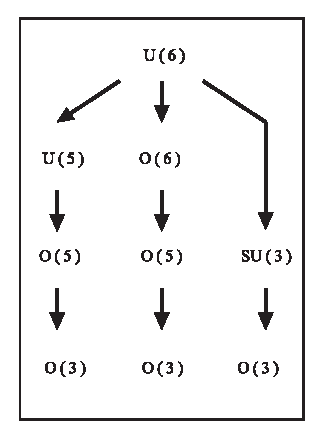
\includegraphics[height=4cm]{figure.eps}
%
% If not, use
%\picplace{5cm}{2cm} % Give the correct figure height and width in cm
%
\caption{Please write your figure caption here}
\label{fig:1}       % Give a unique label
\end{figure}
%
% For built-in environments use
%
\begin{theorem}
Theorem text goes here.
\end{theorem}
%
% or
%
\begin{lemma}
Lemma text goes here.
\end{lemma}
%
%
% Problems or Exercises should be sorted chapterwise
\section*{Problems}
\addcontentsline{toc}{section}{Problems}
%
% Use the following environment.
% Don't forget to label each problem;
% the label is needed for the solutions' environment
\begin{prob}
\label{prob1}
The problem\footnote{Footnote} is described here. The
problem is described here. The problem is described here.
\end{prob}

\begin{prob}
\label{prob2}
\textbf{Problem Heading}\\
(a) The first part of the problem is described here.\\
(b) The second part of the problem is described here.
\end{prob}



%

%%%%%%%%%%%%%%%%%%%%%% chapter.tex %%%%%%%%%%%%%%%%%%%%%%%%%%%%%%%%%
%
% sample chapter
%
% Use this file as a template for your own input.
%
%%%%%%%%%%%%%%%%%%%%%%%% Springer-Verlag %%%%%%%%%%%%%%%%%%%%%%%%%%

\chapter{Chapter Heading}
\label{intro} % Always give a unique label
% use \chaptermark{}
% to alter or adjust the chapter heading in the running head

Your text goes here. Separate text sections with the standard \LaTeX\
sectioning commands.

\section{Section Heading}
\label{sec:1}
% Always give a unique label
% and use \ref{<label>} for cross-references
% and \cite{<label>} for bibliographic references
% use \sectionmark{}
% to alter or adjust the section heading in the running head
Your text goes here. Use the \LaTeX\ automatism for your citations
\cite{monograph}.

\subsection{Subsection Heading}
\label{sec:2}
Your text goes here.

\begin{equation}
\vec{a}\times\vec{b}=\vec{c}
\end{equation}

\subsubsection{Subsubsection Heading}
Your text goes here. Use the \LaTeX\ automatism for cross-references as
well as for your citations, see Sect.~\ref{sec:1}.

\paragraph{Paragraph Heading} %
Your text goes here.

\subparagraph{Subparagraph Heading.} Your text goes here.%
%
\index{paragraph}
% Use the \index{} command to code your index words
%
% For tables use
%
\begin{table}
\centering
\caption{Please write your table caption here}
\label{tab:1}       % Give a unique label
%
% For LaTeX tables use
%
\begin{tabular}{lll}
\hline\noalign{\smallskip}
first & second & third  \\
\noalign{\smallskip}\hline\noalign{\smallskip}
number & number & number \\
number & number & number \\
\noalign{\smallskip}\hline
\end{tabular}
\end{table}
%
%
% For figures use
%
\begin{figure}
\centering
% Use the relevant command for your figure-insertion program
% to insert the figure file.
% For example, with the option graphics use
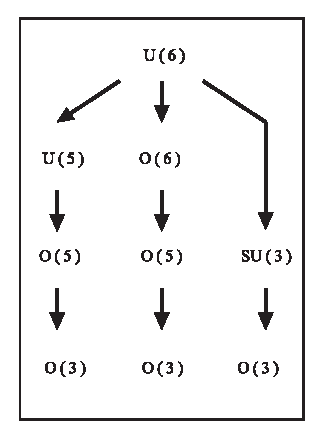
\includegraphics[height=4cm]{figure.eps}
%
% If not, use
%\picplace{5cm}{2cm} % Give the correct figure height and width in cm
%
\caption{Please write your figure caption here}
\label{fig:1}       % Give a unique label
\end{figure}
%
% For built-in environments use
%
\begin{theorem}
Theorem text goes here.
\end{theorem}
%
% or
%
\begin{lemma}
Lemma text goes here.
\end{lemma}
%
%
% Problems or Exercises should be sorted chapterwise
\section*{Problems}
\addcontentsline{toc}{section}{Problems}
%
% Use the following environment.
% Don't forget to label each problem;
% the label is needed for the solutions' environment
\begin{prob}
\label{prob1}
The problem\footnote{Footnote} is described here. The
problem is described here. The problem is described here.
\end{prob}

\begin{prob}
\label{prob2}
\textbf{Problem Heading}\\
(a) The first part of the problem is described here.\\
(b) The second part of the problem is described here.
\end{prob}



%

%\appendix
%\include{appendix}

\backmatter%%%%%%%%%%%%%%%%%%%%%%%%%%%%%%%%%%%%%%%%%%%%%%%%%%%%%%%

\chapter*{Solutions}
\addcontentsline{toc}{chapter}{Solutions}
\markboth{Solutions}{Solutions}

\section*{Problems of Chapter~\ref{intro}}

\begin{sol}{prob1}
The solution is revealed here.
\end{sol}


\begin{sol}{prob2}
\textbf{Problem Heading}\\
(a) The solution of first part is revealed here.\\
(b) The solution of second part is revealed here.
\end{sol}


%%%%%%%%%%%%%%%%%%%%%%%% referenc.tex %%%%%%%%%%%%%%%%%%%%%%%%%%%%%%
% sample references
% "computer science"
%
% Use this file as a template for your own input.
%
%%%%%%%%%%%%%%%%%%%%%%%% Springer-Verlag %%%%%%%%%%%%%%%%%%%%%%%%%%

%
% BibTeX users please use
% \bibliographystyle{}
% \bibliography{}
%
% Non-BibTeX users please use
\begin{thebibliography}{99.}
%
% and use \bibitem to create references.
%
% Use the following syntax and markup for your references
%
% Monographs
\bibitem{monograph} Kajan E (2002)
Information technology encyclopedia and acronyms. Springer, Berlin
Heidelberg New York

% Contributed Works
\bibitem{contribution} Broy M (2002) Software engineering -- From
auxiliary to key technologies. In: Broy M, Denert E (eds)
Software Pioneers. Springer, Berlin Heidelberg New York

% Journal
\bibitem{journal} Che M, Grellmann W, Seidler S (1997)
Appl Polym Sci 64:1079--1090

% Theses
\bibitem{thesis} Ross DW (1977) Lysosomes and storage diseases. MA
Thesis, Columbia University, New York

\end{thebibliography}

\printindex

%%%%%%%%%%%%%%%%%%%%%%%%%%%%%%%%%%%%%%%%%%%%%%%%%%%%%%%%%%%%%%%%%%%%%%

\end{document}





